\PassOptionsToPackage{table}{xcolor}
\documentclass[aspectratio=169]{beamer}\usepackage[utf8]{inputenc}
\usepackage{lmodern}
\usepackage[english]{babel}
\usepackage{color}
\usepackage{amsmath,mathtools}
\usepackage{booktabs}
\usepackage{mathptmx}
\usepackage[11pt]{moresize}
\usepackage{hyperref}
\usepackage{commath}
\usepackage{bm}
\usepackage{subfigure}
\usepackage{siunitx}

\setbeamertemplate{navigation symbols}{}
\setbeamersize{text margin left=5mm,text margin right=5mm}
\setbeamertemplate{caption}[numbered]
\addtobeamertemplate{navigation symbols}{}{
\usebeamerfont{footline}
\usebeamercolor[fg]{footline}
\hspace{1em}
\insertframenumber/\inserttotalframenumber}

\newcommand{\R}{\mathbb{R}}
\newcommand{\E}{\mathbb{E}}
\newcommand{\N}{\mathbb{N}}
\newcommand{\Z}{\mathbb{Z}}
\newcommand{\V}{\mathbb{V}}
\newcommand{\Q}{\mathbb{Q}}
\newcommand{\K}{\mathbb{K}}
\newcommand{\C}{\mathbb{C}}
\newcommand{\T}{\mathbb{T}}
\newcommand{\I}{\mathbb{I}}
\DeclareMathOperator{\sign}{sign}

\title{Summary of Advances and Questions}
\subtitle{Renzo Miguel Caballero Rosas}

\begin{document}

\begin{frame}
\titlepage
\end{frame}

%%%%%%%%%%%%%%%%%%%%%%%%%%%%%%%%%%%%%%%%%%%%%%%%%%%

\setbeamercolor{background canvas}{bg=green!20}
\begin{frame}

{\Huge Error SDE (process $V_t=X_t-p_t$):}

\end{frame}

%%%%%%%%%%%%%%%%%%%%%%%%%%%%%%%%%%%%%%%%%%%%%%%%%%%

\setbeamercolor{background canvas}{bg=white!10}
\begin{frame}\frametitle{Parameters inference using MLE:} \label{MLE}

\begin{columns}

\column{.5\textwidth}
On the right, we can see the level sets for the negative log-likelihood. The thick violet band is the region where the function reaches its minimums.\\
\quad\\
We can see the \textbf{initial guess} point, the result of three different \textbf{optimization tools} from MATLAB, and the minimum point that we found from the \textbf{evaluations} that generate the plot.\\
\quad\\
Notice that all the optimal locations are in the minimum value band.

\column{.5\textwidth}
\begin{figure}[ht!]
\centering
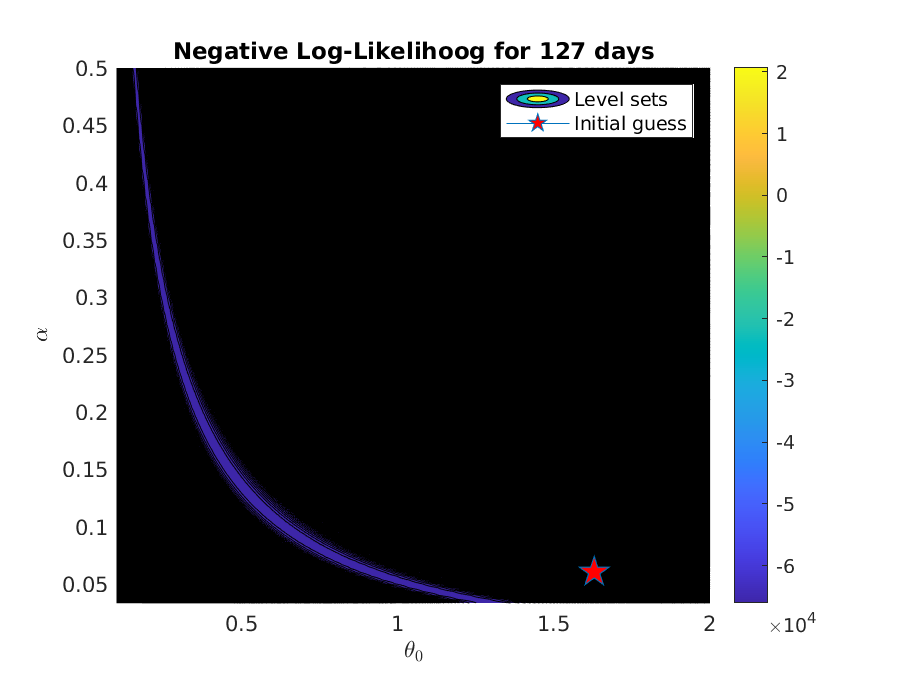
\includegraphics[width=0.85\textwidth]{../../MATLAB_Files/Results/likelihood/normal/Log-Likelihood.eps}\\
{\tiny
\begin{table}[]
\begin{tabular}{lccc}
\toprule
 & $\theta_0$ & $\alpha$ & $\theta_0\alpha$\\
 \midrule
 Initial guess & 1.629 & 0.060 & 0.098 \\
 fminsearch & 1.135 & 0.073 & 0.083 \\
 fmincon & 1.366 & 0.061 & 0.083 \\
 fminunc & 1.628 & 0.051 & 0.083 \\
 evaluations & 1.180 & 0.070 & 0.083 \\
 \bottomrule
\end{tabular}
\end{table}
}
\end{figure}

\end{columns}

\end{frame}

%%%%%%%%%%%%%%%%%%%%%%%%%%%%%%%%%%%%%%%%%%%%%%%%%%%

\setbeamercolor{background canvas}{bg=white!10}
\begin{frame}\frametitle{Some key points:}

\begin{enumerate}

\item The moments' ODEs were verified with the empirical moments using Euler–Maruyama method.
\item All the optimization tools are set to their default specifications. However, if we increment the precision of the tools, or if we normalize the likelihood, we do not see significant changes in the position of the minimums.
\item All the minimums are over the line $\theta_0\alpha=0.083$. This line is exactly located in the center of the thick violet band.
\item We do inference using 127 days ('training days'), and simulate over the other 128 days ('testing days'). In total, we have  255 days, since we removed all the days with curtailing. To guarantee independence between the days, we never do inference using two consecutive (in the calendar sense) days.

\end{enumerate}
\alert{If there is any question, please let me know.}
\end{frame}

%%%%%%%%%%%%%%%%%%%%%%%%%%%%%%%%%%%%%%%%%%%%%%%%%%%

\setbeamercolor{background canvas}{bg=white!10}
\begin{frame}\frametitle{More evaluations:}

\begin{figure}[ht!]
\centering
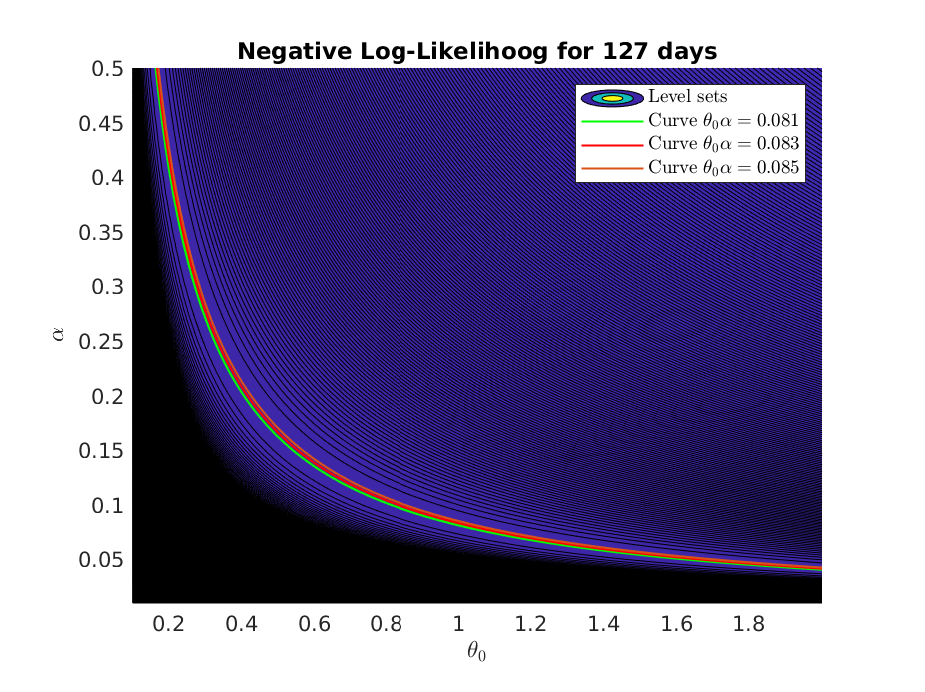
\includegraphics[width=0.5\textwidth]{../../MATLAB_Files/Results/likelihood/normal/Log-Likelihood_Line.eps}
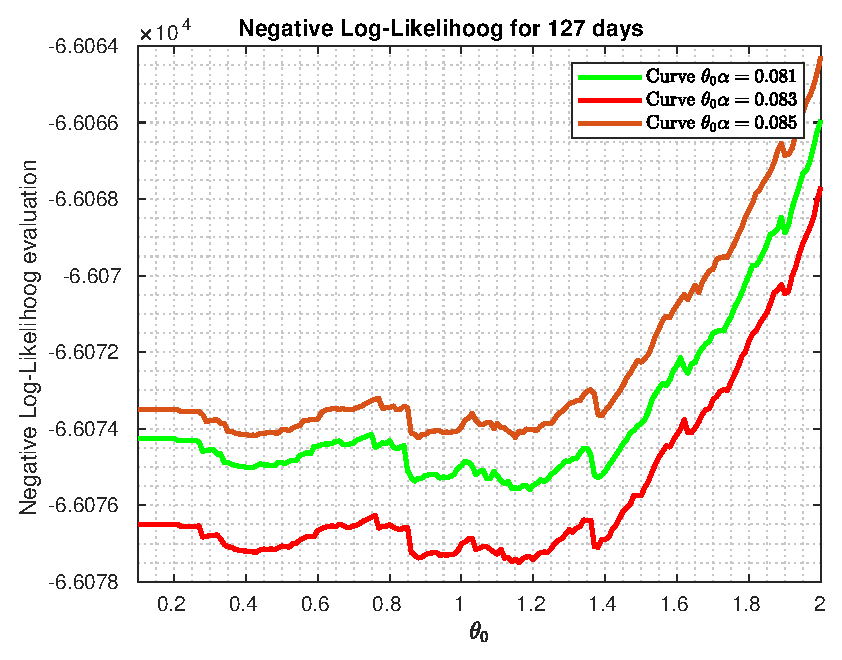
\includegraphics[width=0.45\textwidth]{../../MATLAB_Files/Results/likelihood/normal/Log-Likelihood_Evaluations.eps}
\end{figure}

We can see that the line $\theta_0\alpha=0.083$ presents the smallest evaluations.

\end{frame}

%%%%%%%%%%%%%%%%%%%%%%%%%%%%%%%%%%%%%%%%%%%%%%%%%%%

\setbeamercolor{background canvas}{bg=white!10}
\begin{frame}\frametitle{Simulations over testing days:}

\begin{figure}[ht!]
\centering
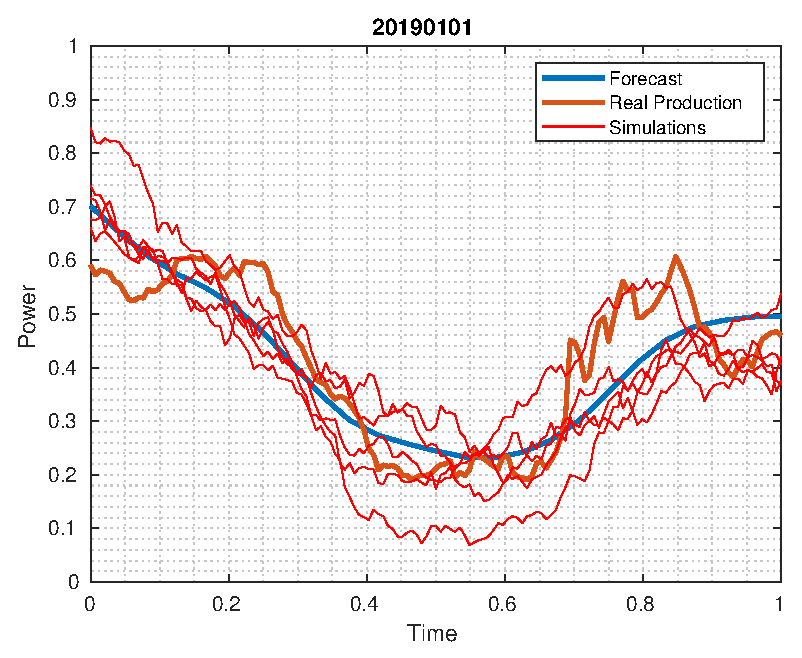
\includegraphics[width=0.3\textwidth]{../../MATLAB_Files/Results/paths_testing_days/optimal_value/1.eps}
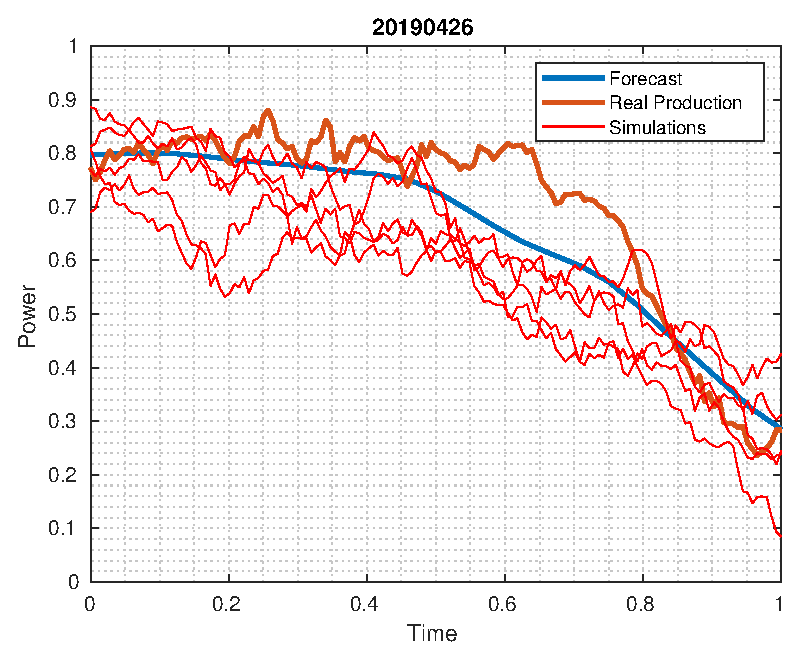
\includegraphics[width=0.3\textwidth]{../../MATLAB_Files/Results/paths_testing_days/optimal_value/2.eps}
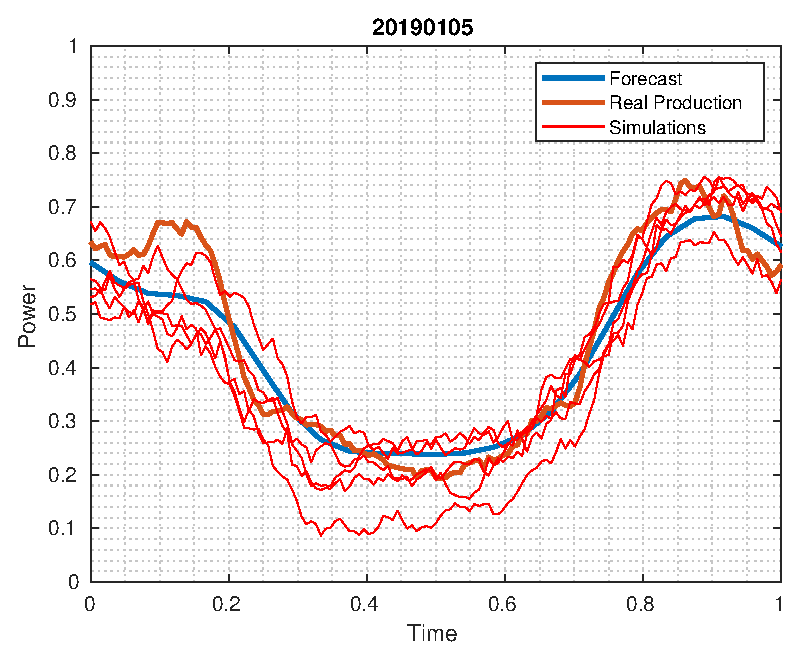
\includegraphics[width=0.3\textwidth]{../../MATLAB_Files/Results/paths_testing_days/optimal_value/3.eps}
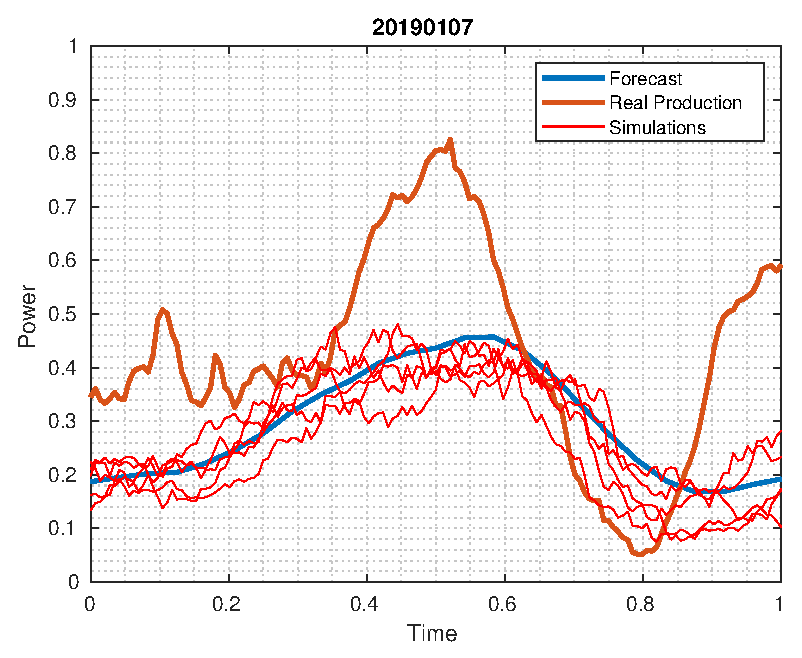
\includegraphics[width=0.3\textwidth]{../../MATLAB_Files/Results/paths_testing_days/optimal_value/4.eps}
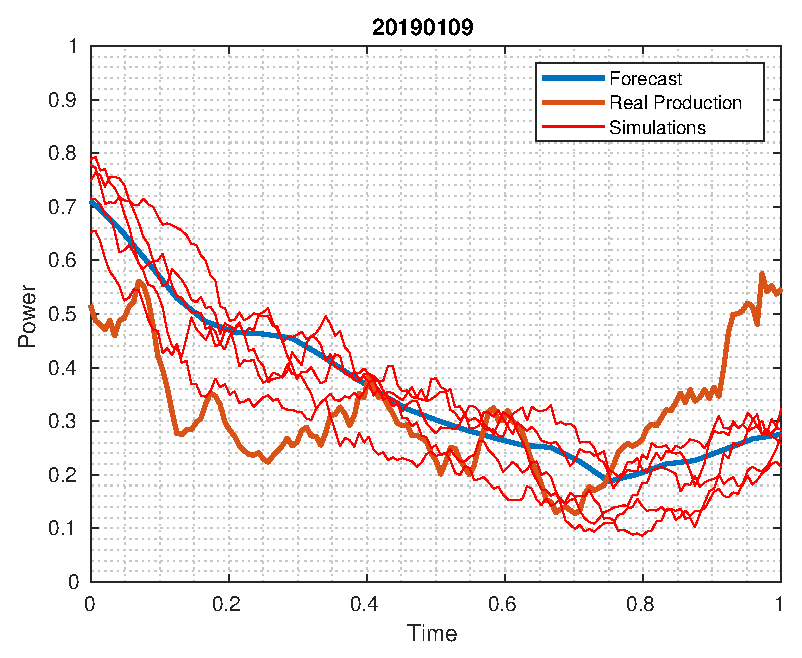
\includegraphics[width=0.3\textwidth]{../../MATLAB_Files/Results/paths_testing_days/optimal_value/5.eps}
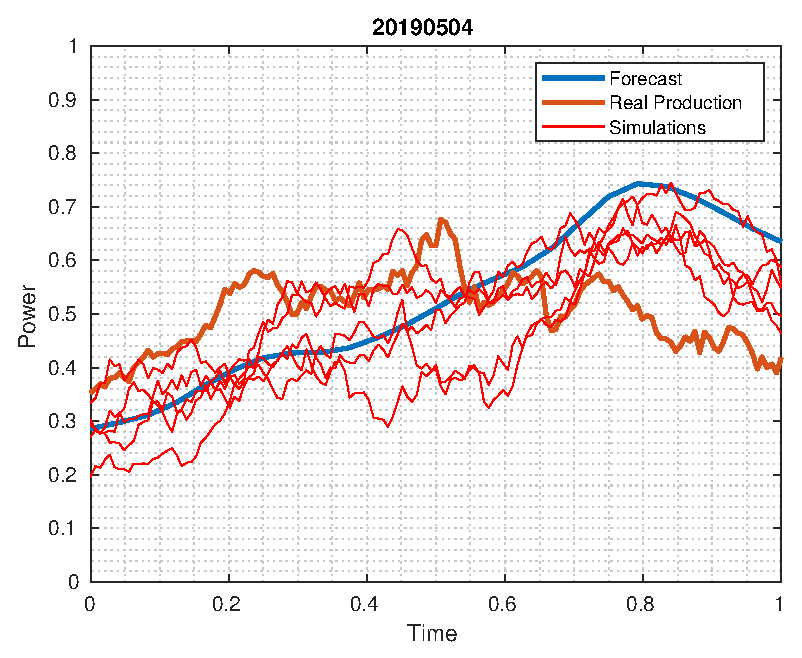
\includegraphics[width=0.3\textwidth]{../../MATLAB_Files/Results/paths_testing_days/optimal_value/6.eps}
\end{figure}

\end{frame}

%%%%%%%%%%%%%%%%%%%%%%%%%%%%%%%%%%%%%%%%%%%%%%%%%%%

\setbeamercolor{background canvas}{bg=white!10}
\begin{frame}\frametitle{Simulations over testing days:}

\begin{figure}[ht!]
\centering
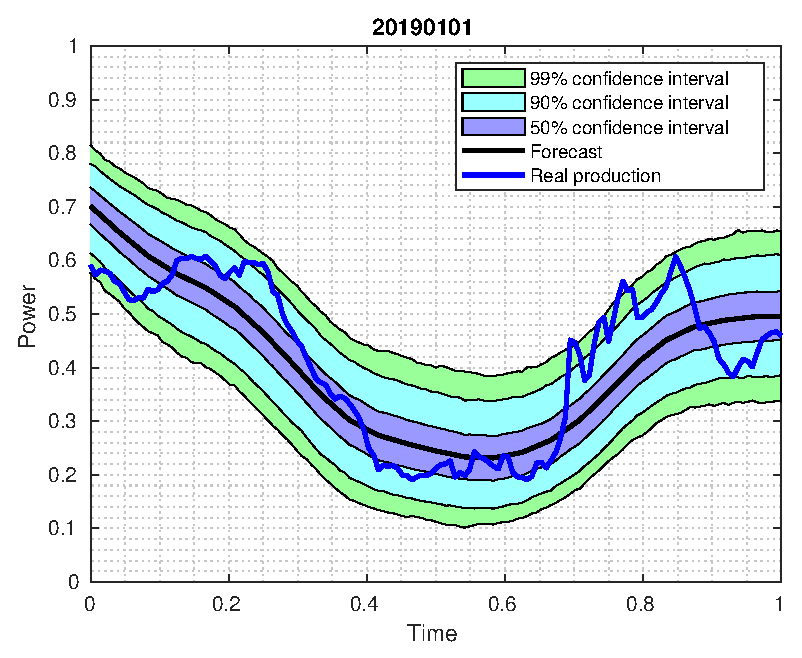
\includegraphics[width=0.3\textwidth]{../../MATLAB_Files/Results/bands_testing_days/optimal_value/1.eps}
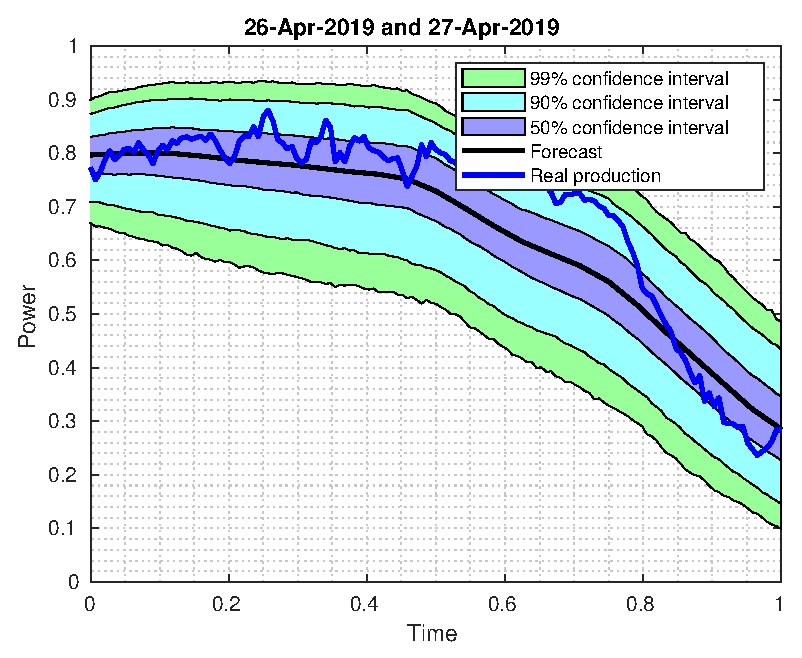
\includegraphics[width=0.3\textwidth]{../../MATLAB_Files/Results/bands_testing_days/optimal_value/2.eps}
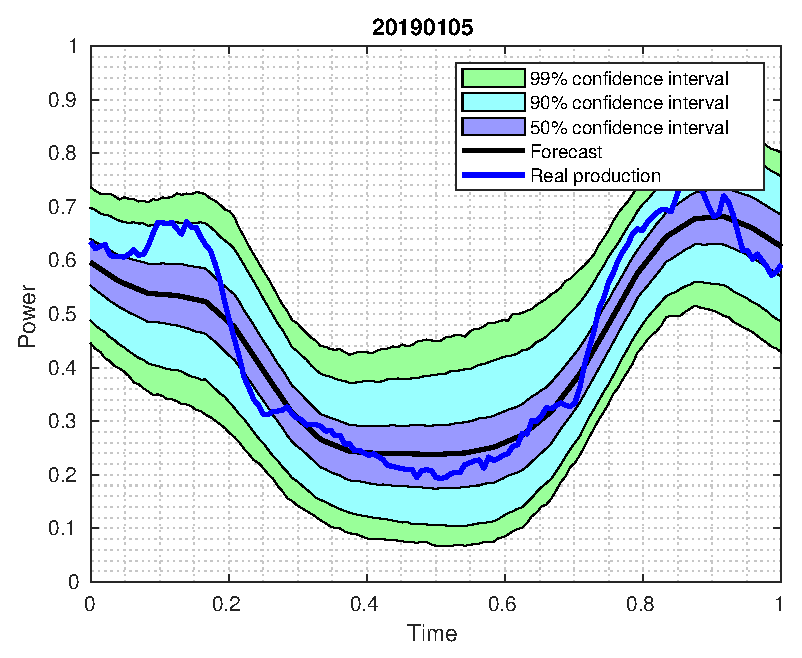
\includegraphics[width=0.3\textwidth]{../../MATLAB_Files/Results/bands_testing_days/optimal_value/3.eps}
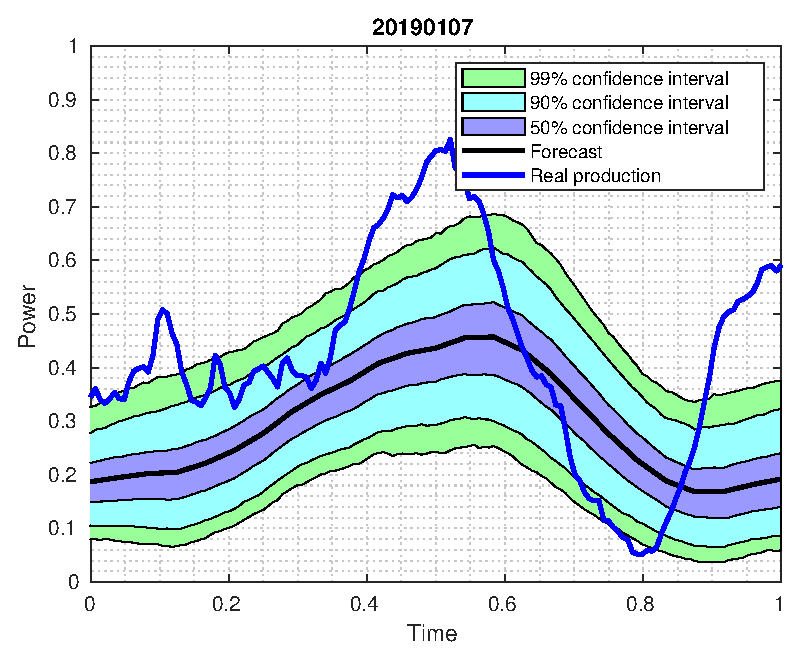
\includegraphics[width=0.3\textwidth]{../../MATLAB_Files/Results/bands_testing_days/optimal_value/4.eps}
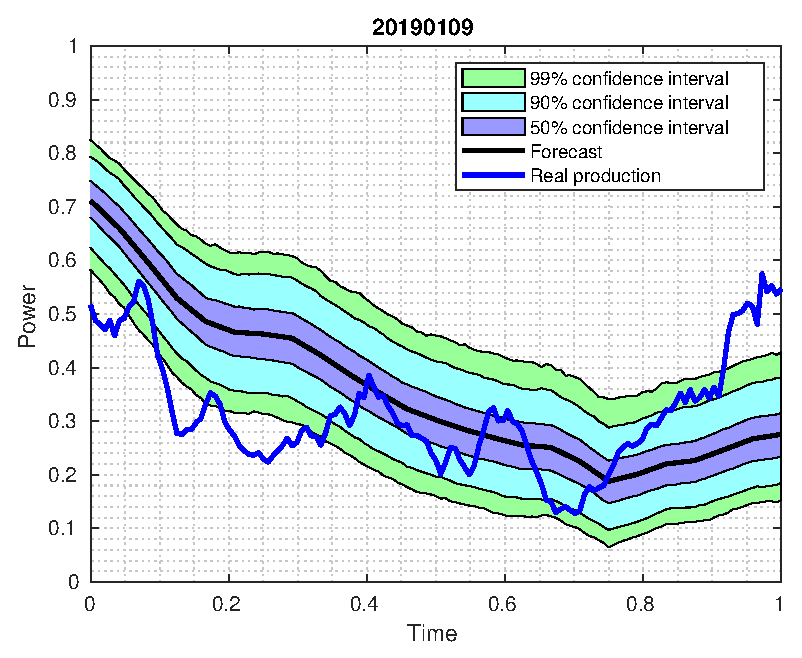
\includegraphics[width=0.3\textwidth]{../../MATLAB_Files/Results/bands_testing_days/optimal_value/5.eps}
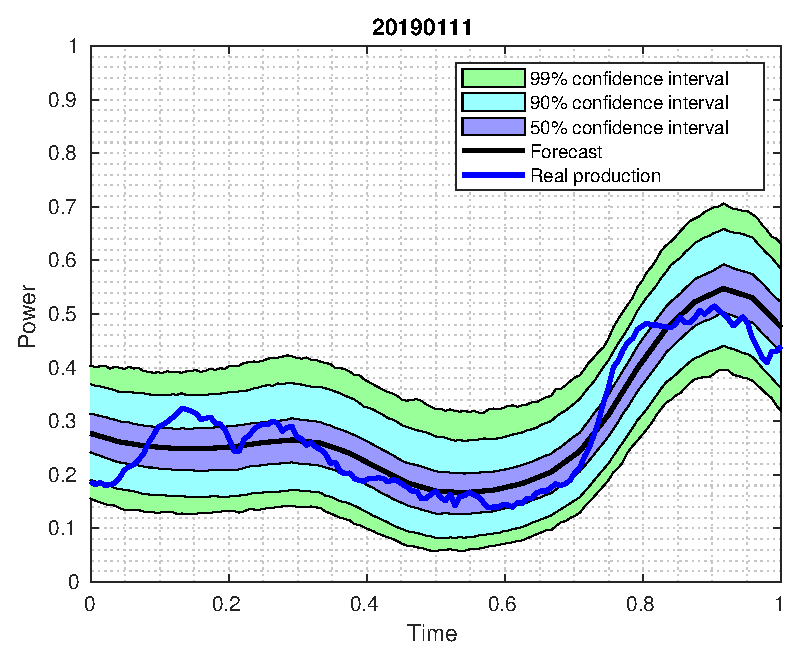
\includegraphics[width=0.3\textwidth]{../../MATLAB_Files/Results/bands_testing_days/optimal_value/6.eps}
\end{figure}

\end{frame}

%%%%%%%%%%%%%%%%%%%%%%%%%%%%%%%%%%%%%%%%%%%%%%%%%%%

\setbeamercolor{background canvas}{bg=white!10}
\begin{frame}\frametitle{Histogram over testing days:}

\begin{columns}

\column{.4\textwidth}
On the right, we can see the histogram of the transition error for the testing days, and the histogram of the simulated transition error over the testing days.\\
\quad\\
We simulated the error SDE using Euler-Maruyama and using $\Delta t=\SI{10}{\min}$.\\
\quad\\
We may achieve more variance than needed because of the fat tail of the original data. Many error transitions are large, and they complicate the inference.

\column{.6\textwidth}
\begin{figure}[ht!]
\centering
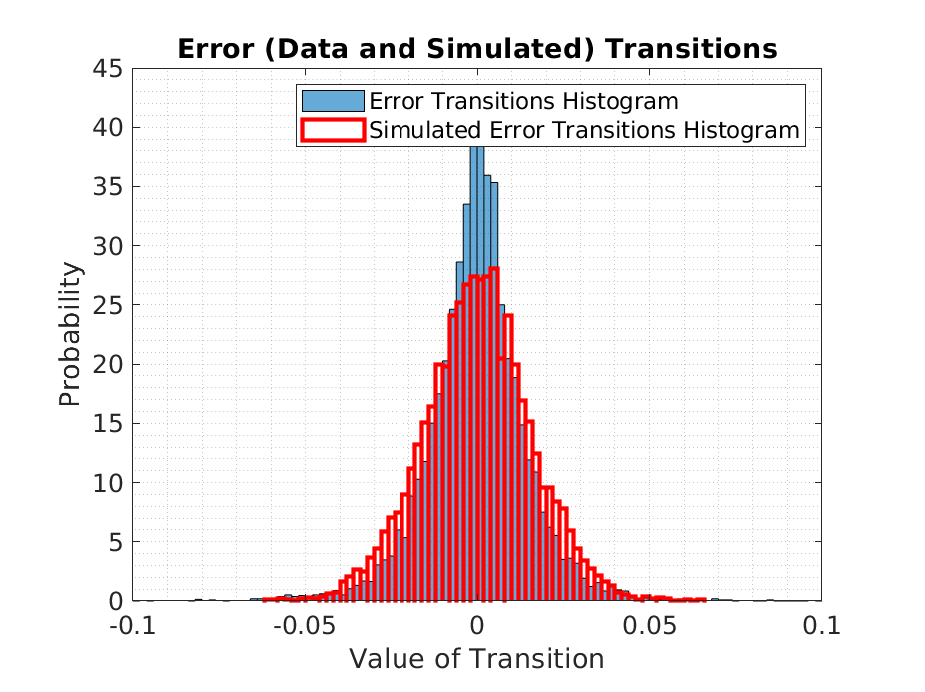
\includegraphics[width=1\textwidth]{../../MATLAB_Files/Results/histograms/classic/Optimal.eps}
\end{figure}

\end{columns}

\end{frame}

%%%%%%%%%%%%%%%%%%%%%%%%%%%%%%%%%%%%%%%%%%%%%%%%%%%

\setbeamercolor{background canvas}{bg=green!20}
\begin{frame}

{\Huge Lamperti Transform (process $Z_t=\psi(V_t)$):}

\end{frame}

%%%%%%%%%%%%%%%%%%%%%%%%%%%%%%%%%%%%%%%%%%%%%%%%%%%

\setbeamercolor{background canvas}{bg=white!10}
\begin{frame}\frametitle{About Lamperti:}

Let $\{\Delta V_i\}_{i=1}^n$ be the set of all error transitions, and $\psi(\theta_0,\alpha,\Delta V)$ the Lamperti transform. Notice that the Lamperti transitions $\{\Delta Z_i\}_{i=1}^n$ depend on $(\theta_0,\alpha)$ because $$\{\Delta Z_i\}_{i=1}^n=\psi(\theta_0,\alpha,\{\Delta V_i\}_{i=1}^n).$$
Then, if we compute $$\max_{(\theta_0,\alpha)}\mathbf{L}(\theta_0,\alpha,\{\Delta Z_i\}_{i=1}^n),$$
we are not computing a MLE in the classical sense, as the data is changing with the parameters. However, we can try to find a fixed point ${\color{blue}(\theta_0^*,\alpha^*)}$ such that
\begin{equation}
{\color{blue}(\theta_0^*,\alpha^*)}=\arg\max_{(\theta_0,\alpha)}\mathbf{L}\left(\theta_0,\alpha,\psi({\color{blue}\theta_0^*},{\color{blue}\alpha^*},\{\Delta V_i\}_{i=1}^n)\right).
\label{FP}
\end{equation}
In this point, the likelihood has a maximum for the data set corresponding to that point. \alert{Does this approach have sense?}

\end{frame}

%%%%%%%%%%%%%%%%%%%%%%%%%%%%%%%%%%%%%%%%%%%%%%%%%%%

\setbeamercolor{background canvas}{bg=white!10}
\begin{frame}\frametitle{Fixed point function:}

We are interested in finding the solution of (\ref{FP}). We have that, if $(\theta_0^*,\alpha^*)$ is a solution of (\ref{FP}), then
\begin{equation*}
(\theta_0^*,\alpha^*)-\arg\max_{(\theta_0,\alpha)}\mathbf{L}\left(\theta_0,\alpha,\psi({\color{black}\theta_0^*},{\color{black}\alpha^*},\{\Delta V_i\}_{i=1}^n)\right)=0.
\end{equation*}
Given a pair $(\theta_0^{*},\alpha^{*})$, we call $(\theta_0^{**},\alpha^{**})$ to the solution of
\begin{equation*}
\arg\max_{(\theta_0,\alpha)}\mathbf{L}\left(\theta_0,\alpha,\psi({\color{black}\theta_0^*},{\color{black}\alpha^*},\{\Delta V_i\}_{i=1}^n)\right).
\end{equation*}
For each $(\theta_0^{*},\alpha^{*})$, we define the relative error function
\begin{equation*}
\Psi(\theta_0^{*},\alpha^{*})=\frac{|\theta_0^{*}-\theta_0^{**}|}{|\theta_0^{*}|}+\frac{|\alpha^{*}-\alpha^{**}|}{|\alpha^{*}|}
\end{equation*}
and claim that $(\theta_0^*,\alpha^*)$ is a fixed point iff $\Psi(\theta_0^*,\alpha^*)=0$.

\end{frame}

%%%%%%%%%%%%%%%%%%%%%%%%%%%%%%%%%%%%%%%%%%%%%%%%%%%+

\setbeamercolor{background canvas}{bg=white!10}
\begin{frame}\frametitle{Fixed point function:}

\begin{columns}

\column{.5\textwidth}
On the right, we can see the numerical level sets of the error function $\Psi$.\\
\quad\\
The center deep green band is the set $\mathbb{A}$ such that $\Psi(\mathbb{A})\in[0.05,0.1]$. We do not achieve relative error smaller than 0.05.\\
\quad\\
We observe a particular behavior over the curves $\theta_0\alpha=k\in\R^+$. However, it can be a numeric effect.\\
\quad\\
We also observe that: $$\mathbb{A}\cap\{(\theta_0,\alpha):\theta_0\alpha=0.083\}\neq\emptyset.$$

\column{.5\textwidth}
\begin{figure}[ht!]
\centering
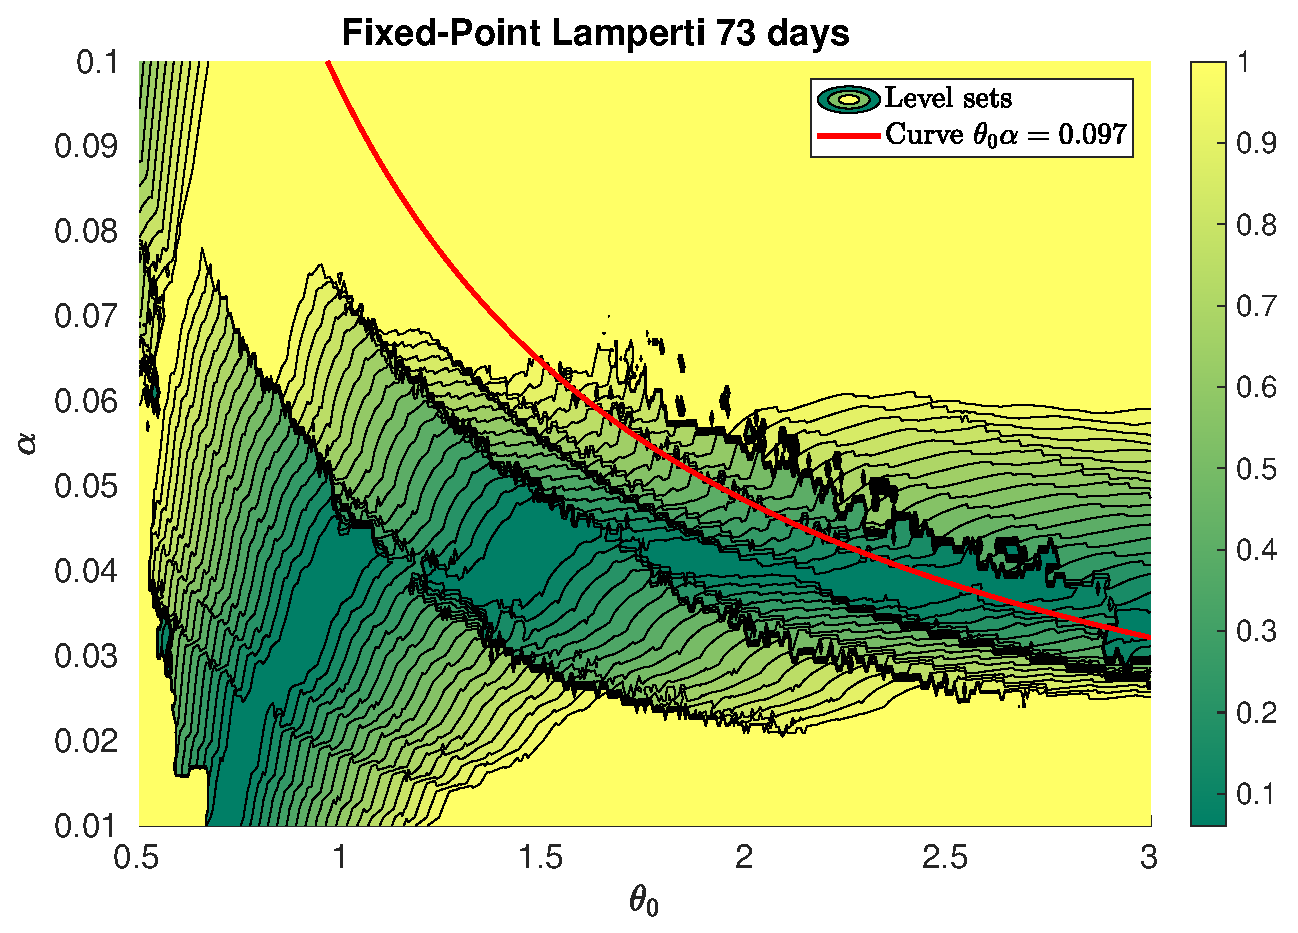
\includegraphics[width=1\textwidth]{../../MATLAB_Files/Results/likelihood/lamperti/Log-Likelihood.eps}
\end{figure}

\end{columns}

\end{frame}

%%%%%%%%%%%%%%%%%%%%%%%%%%%%%%%%%%%%%%%%%%%%%%%%%%%+

\setbeamercolor{background canvas}{bg=white!10}
\begin{frame}\frametitle{Fixed point function:}

\begin{columns}

\column{.5\textwidth}
On the right, we observe some possible candidates for fixed points, that also satisfies the empirical condition $\theta_0\alpha=0.038$ from the error SDE.\\
\quad\\
We choose $(\theta_0,\alpha)=(2.200,0.038)$.\\
\quad\\
We interpret the set $\mathbb{A}$ as "the points where the transformation of the data, does not interfere with MLE". \alert{Is this interpretation correct?}

\column{.5\textwidth}
\begin{figure}[ht!]
\centering
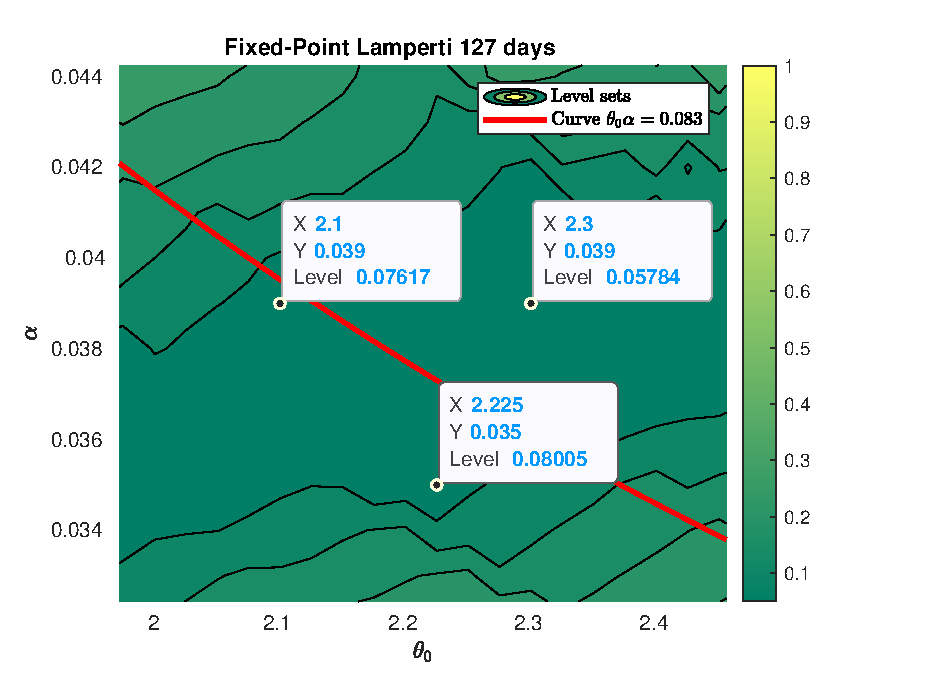
\includegraphics[width=1\textwidth]{../../MATLAB_Files/Results/likelihood/lamperti/Log-Likelihood_2.eps}
\end{figure}

\end{columns}

\end{frame}

%%%%%%%%%%%%%%%%%%%%%%%%%%%%%%%%%%%%%%%%%%%%%%%%%%%

\setbeamercolor{background canvas}{bg=white!10}
\begin{frame}\frametitle{Simulations over testing days:}

\begin{figure}[ht!]
\centering
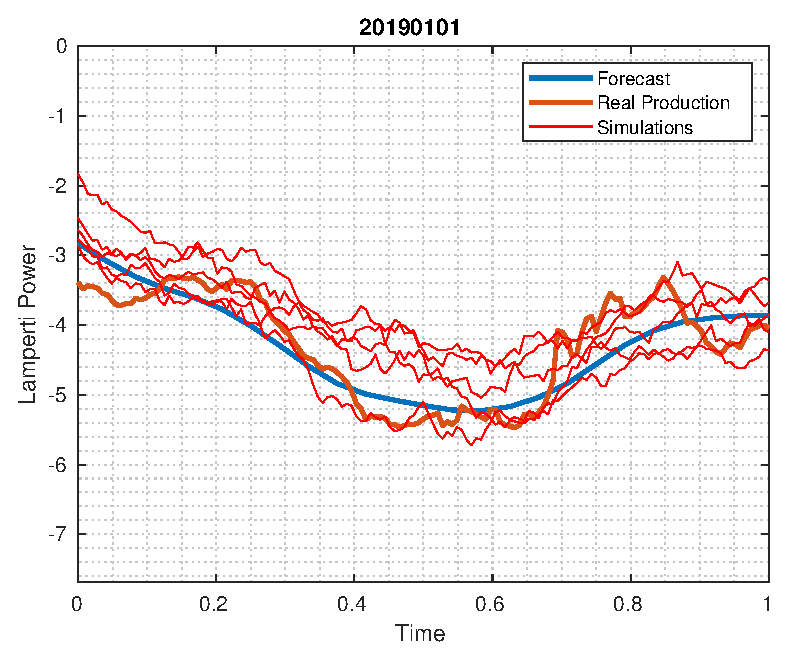
\includegraphics[width=0.3\textwidth]{../../MATLAB_Files/Results/paths_testing_days/lamperti_optimal/1.eps}
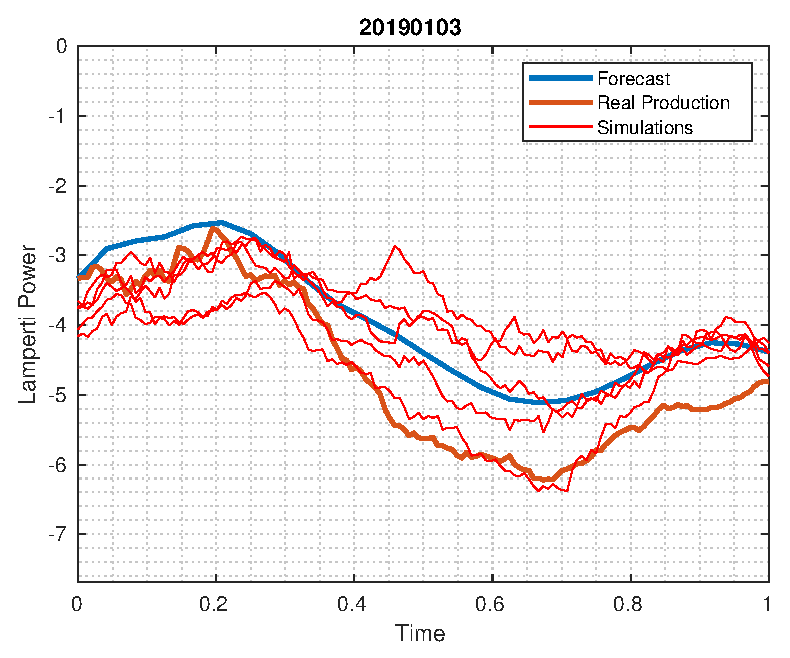
\includegraphics[width=0.3\textwidth]{../../MATLAB_Files/Results/paths_testing_days/lamperti_optimal/2.eps}
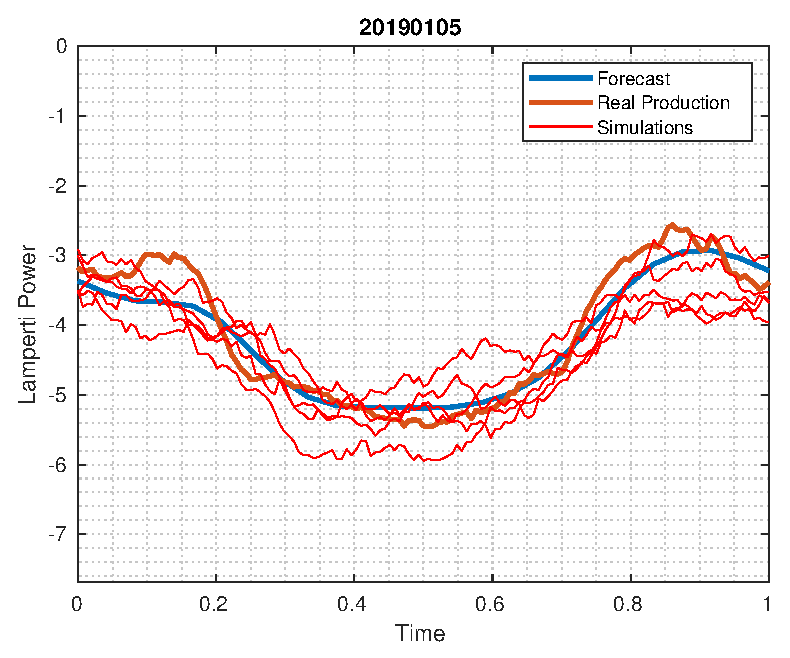
\includegraphics[width=0.3\textwidth]{../../MATLAB_Files/Results/paths_testing_days/lamperti_optimal/3.eps}
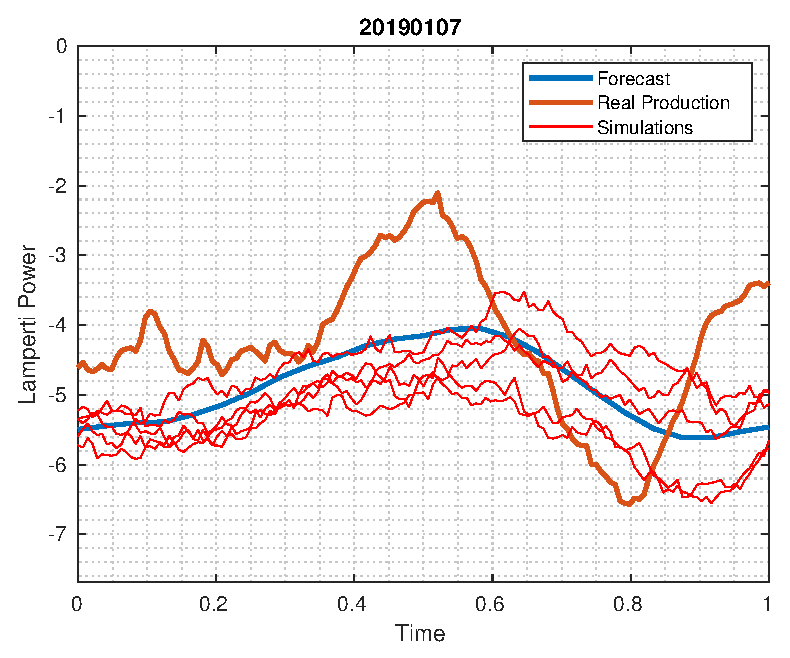
\includegraphics[width=0.3\textwidth]{../../MATLAB_Files/Results/paths_testing_days/lamperti_optimal/4.eps}
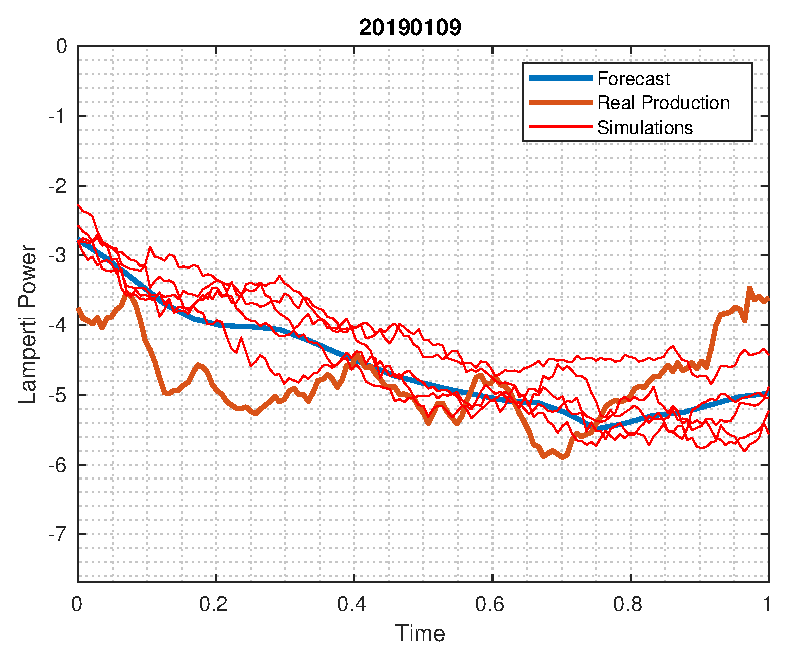
\includegraphics[width=0.3\textwidth]{../../MATLAB_Files/Results/paths_testing_days/lamperti_optimal/5.eps}
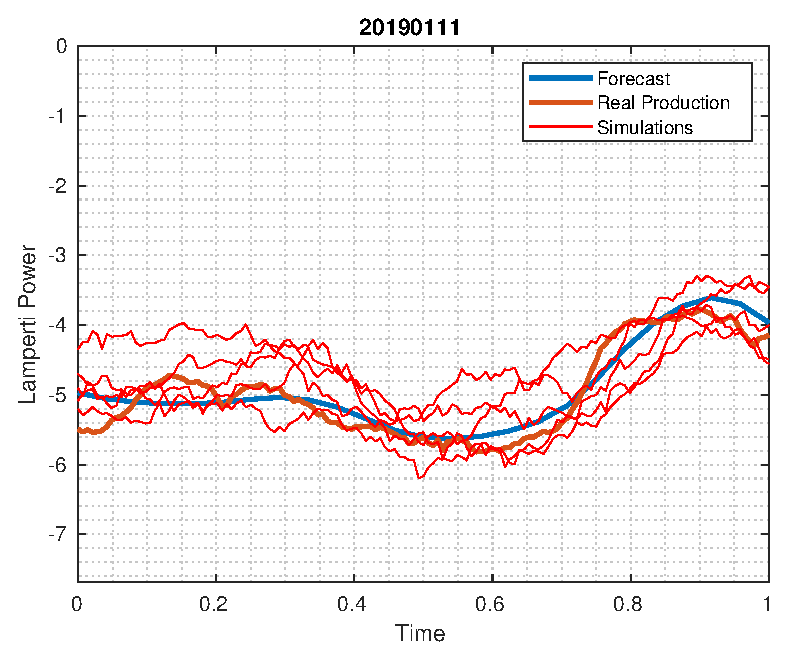
\includegraphics[width=0.3\textwidth]{../../MATLAB_Files/Results/paths_testing_days/lamperti_optimal/6.eps}
\end{figure}

\end{frame}

%%%%%%%%%%%%%%%%%%%%%%%%%%%%%%%%%%%%%%%%%%%%%%%%%%%

\setbeamercolor{background canvas}{bg=white!10}
\begin{frame}\frametitle{Simulations over testing days:}

\begin{figure}[ht!]
\centering
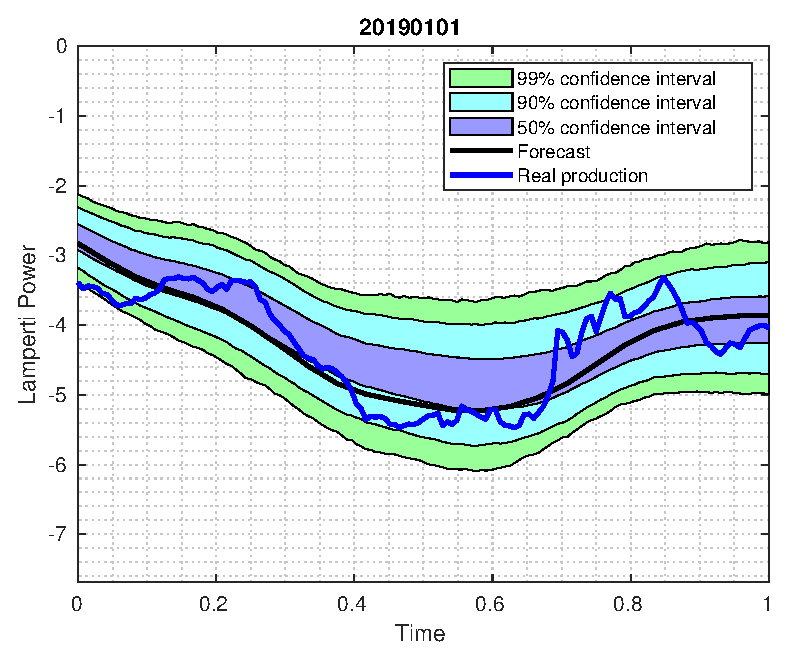
\includegraphics[width=0.3\textwidth]{../../MATLAB_Files/Results/bands_testing_days/lamperti_optimal/1.eps}
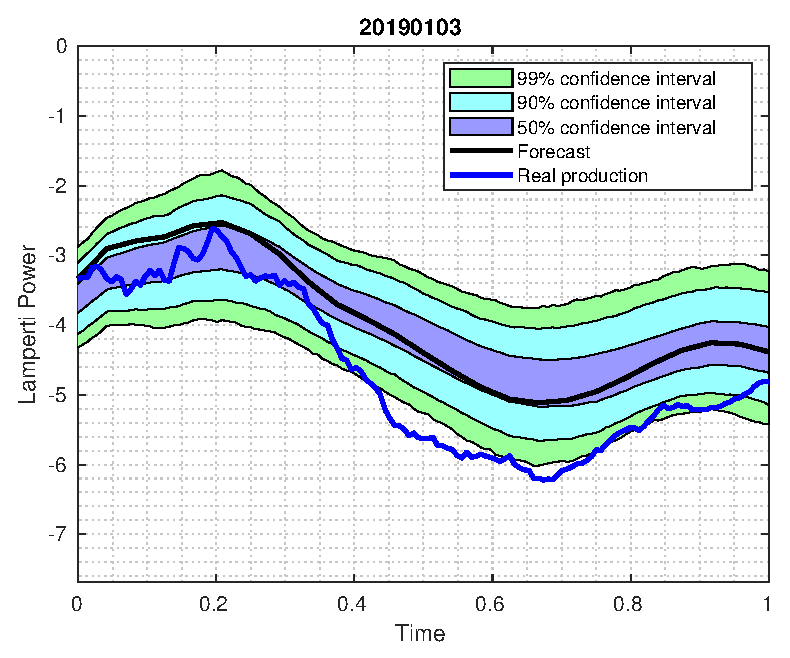
\includegraphics[width=0.3\textwidth]{../../MATLAB_Files/Results/bands_testing_days/lamperti_optimal/2.eps}
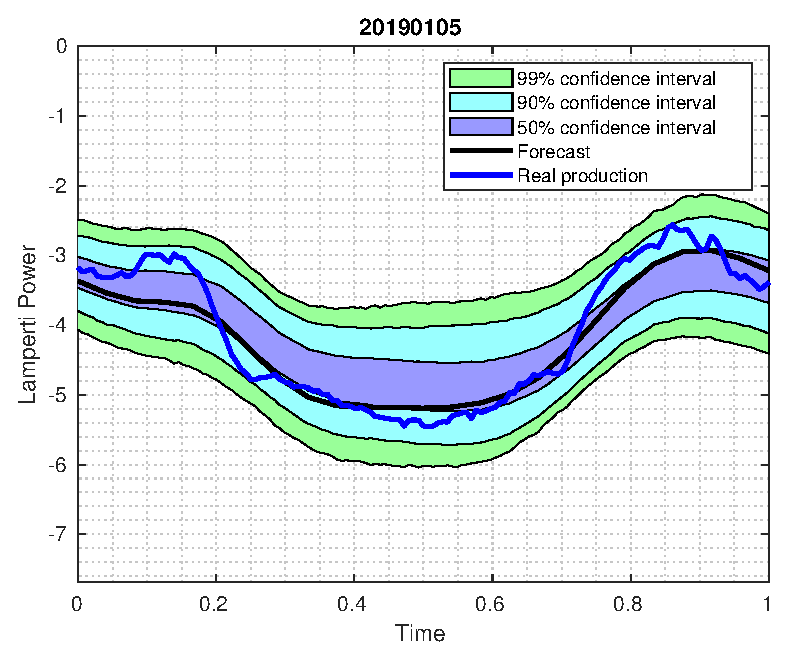
\includegraphics[width=0.3\textwidth]{../../MATLAB_Files/Results/bands_testing_days/lamperti_optimal/3.eps}
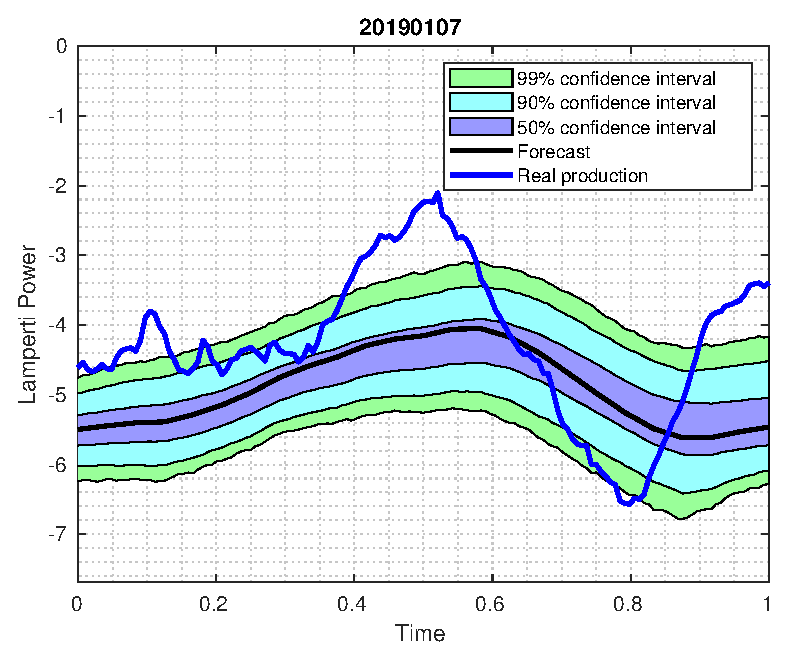
\includegraphics[width=0.3\textwidth]{../../MATLAB_Files/Results/bands_testing_days/lamperti_optimal/4.eps}
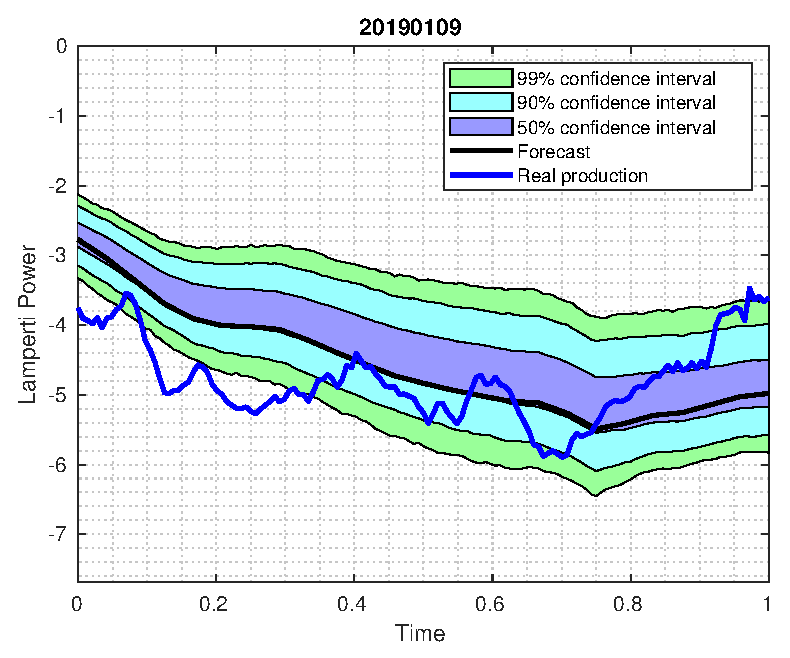
\includegraphics[width=0.3\textwidth]{../../MATLAB_Files/Results/bands_testing_days/lamperti_optimal/5.eps}
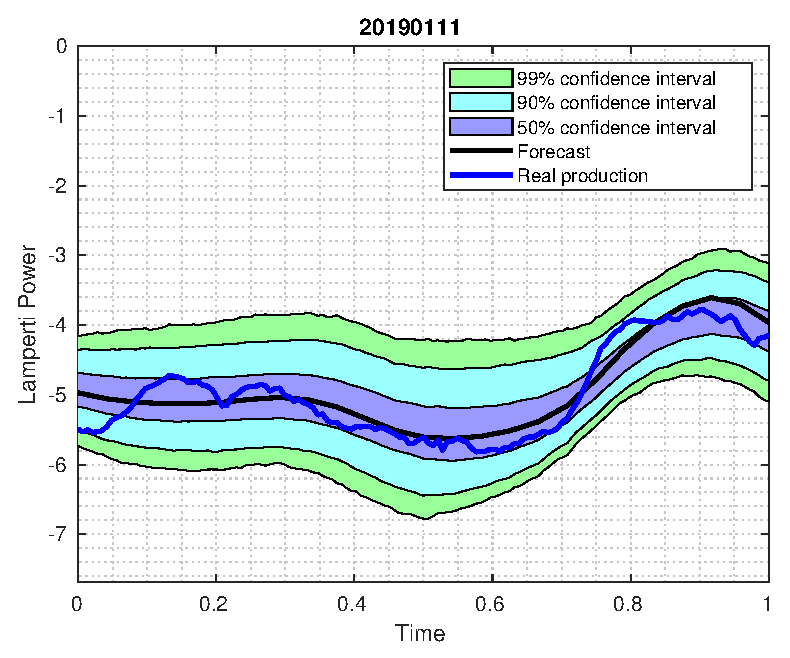
\includegraphics[width=0.3\textwidth]{../../MATLAB_Files/Results/bands_testing_days/lamperti_optimal/6.eps}
\end{figure}

\end{frame}

%%%%%%%%%%%%%%%%%%%%%%%%%%%%%%%%%%%%%%%%%%%%%%%%%%%

\setbeamercolor{background canvas}{bg=white!10}
\begin{frame}\frametitle{Histogram over testing days:}

\begin{columns}

\column{.4\textwidth}
On the right, we can see the histogram of the Lamperti transitions for the testing days, and the histogram of the simulated Lamperti transitions over the testing days.\\
\quad\\
We simulated the Lamperti SDE using Euler-Maruyama and using $\Delta t=\SI{10}{\min}$.

\column{.6\textwidth}
\begin{figure}[ht!]
\centering
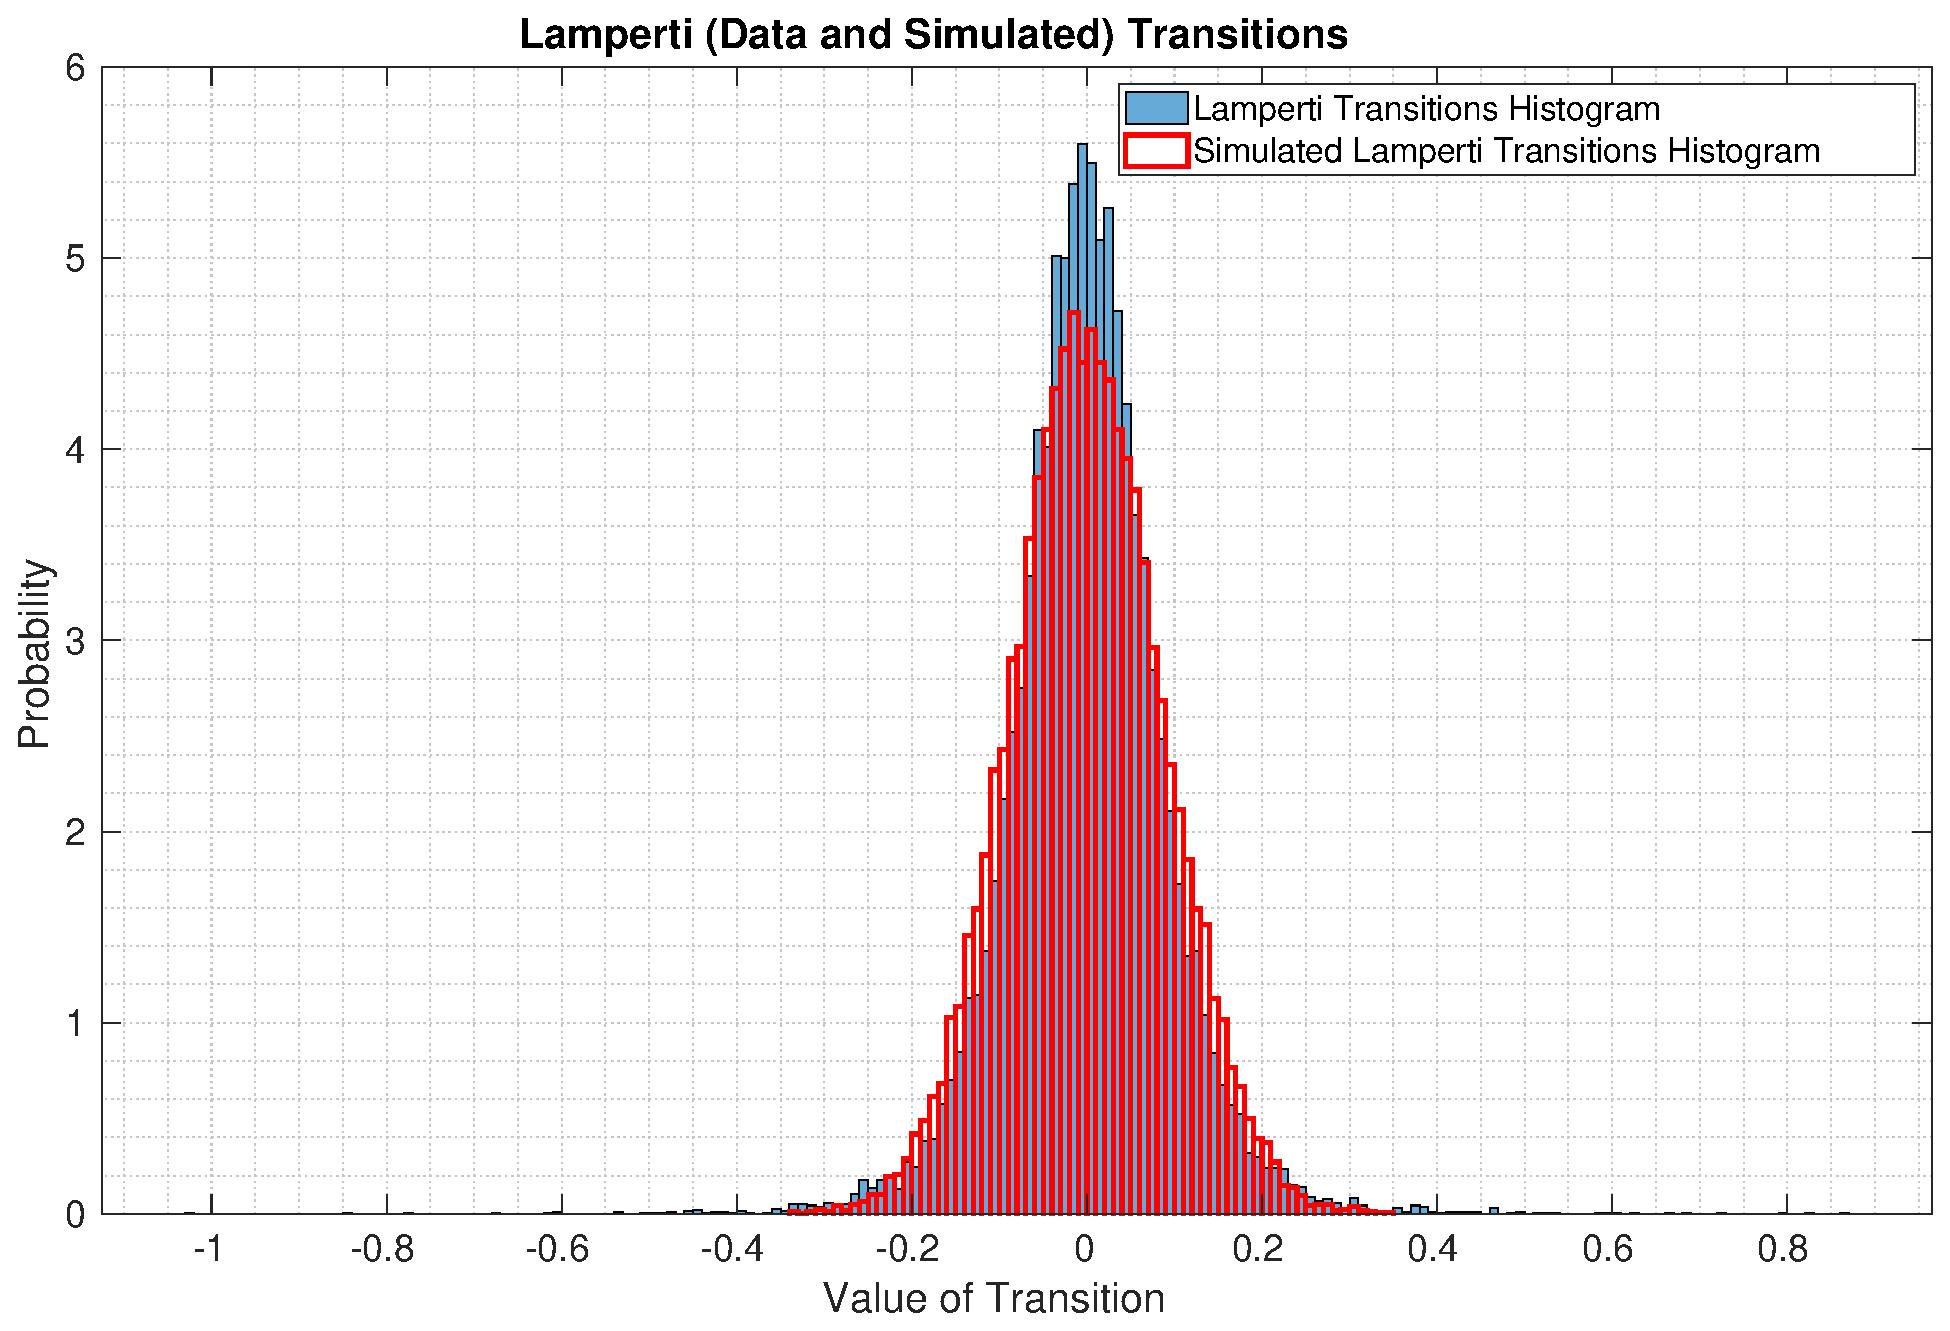
\includegraphics[width=1\textwidth]{../../MATLAB_Files/Results/histograms/lamperti/Optimal_Lamperti.eps}
\end{figure}

\end{columns}

\end{frame}

%%%%%%%%%%%%%%%%%%%%%%%%%%%%%%%%%%%%%%%%%%%%%%%%%%%

\setbeamercolor{background canvas}{bg=white!10}
\begin{frame}\frametitle{Some key points:}

\begin{enumerate}

\item The moments' ODEs were verified with the empirical moments using Euler–Maruyama method.
\item From the set $\mathbb{A}$, we choose a point that satisfies $\theta_0\alpha=0.083$ as it looks to be a necessary condition for the error SDE.
\item We do inference using 127 days ('training days'), and simulate over the other 128 days ('testing days'). In total, we have  255 days, since we removed all the days with curtailing. To guarantee independence between the days, we never do inference using two consecutive (in the calendar sense) days.
\item \alert{Should the bands be centered in the transformed forecast?}
\item \alert{Does this fixed-point method have sense?}
\item The day 07/01/2019 was particularly bad, with a terrible forecast.

\end{enumerate}

\end{frame}

%%%%%%%%%%%%%%%%%%%%%%%%%%%%%%%%%%%%%%%%%%%%%%%%%%%

\setbeamercolor{background canvas}{bg=green!20}
\begin{frame}

{\Huge Two optimal values:}

\end{frame}

%%%%%%%%%%%%%%%%%%%%%%%%%%%%%%%%%%%%%%%%%%%%%%%%%%%

\setbeamercolor{background canvas}{bg=white!10}
\begin{frame}\frametitle{Two optimal values:}

We achieve two possible values for the parameters.
\begin{enumerate}

\item Using inference in the error SDE, we get $(\theta_0^E,\alpha^E)=(1.180,0.070)$.
\item Using our fixed-point method for the Lamperti MLE, and imposing the extra condition $\theta_0\alpha=0.038$, we get $(\theta_0^L,\alpha^L)=(2.200,0.038)$.

\end{enumerate}
\quad\\
\quad\\
\alert{How can we compare which is better? Or even correct?} We will show in the next slides comparative histograms, paths and probability bands. All of them for the original error SDE.

\end{frame}

%%%%%%%%%%%%%%%%%%%%%%%%%%%%%%%%%%%%%%%%%%%%%%%%%%%

\setbeamercolor{background canvas}{bg=white!10}
\begin{frame}\frametitle{Error transitions histograms:}

\begin{figure}[ht!]
\centering
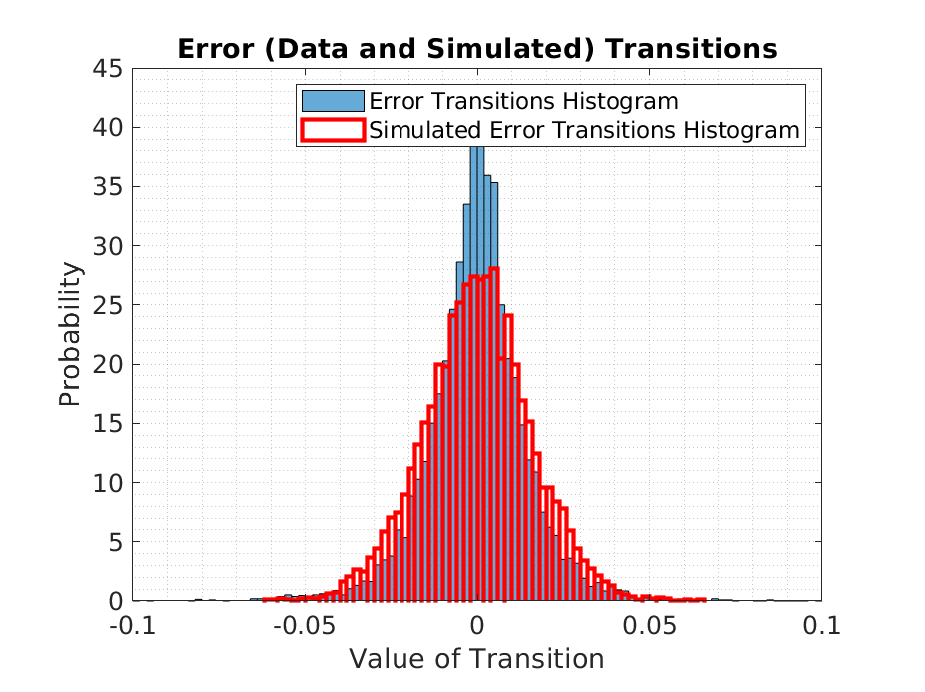
\includegraphics[width=0.48\textwidth]{../../MATLAB_Files/Results/histograms/classic/Optimal.eps}
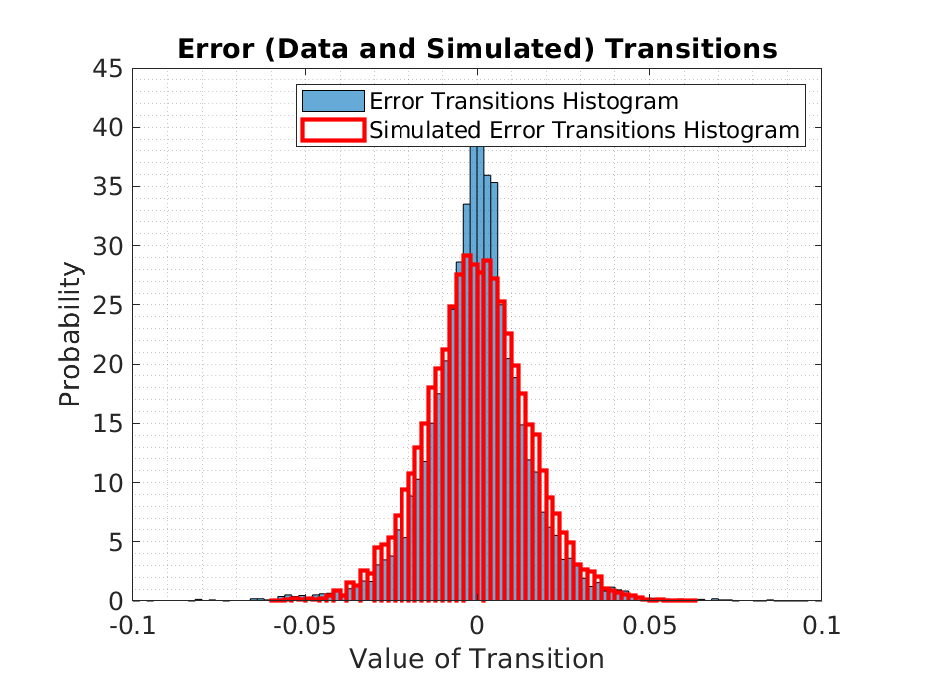
\includegraphics[width=0.48\textwidth]{../../MATLAB_Files/Results/histograms/classic/Lamperti_Optimal.eps}
\end{figure}

We can see two histograms for the error transitions. On the left, using $(\theta_0^E,\alpha^E)$, while on the right, using $(\theta_0^L,\alpha^L)$.

\end{frame}

%%%%%%%%%%%%%%%%%%%%%%%%%%%%%%%%%%%%%%%%%%%%%%%%%%%

\setbeamercolor{background canvas}{bg=white!10}
\begin{frame}\frametitle{Simulations over testing days: First row: $(\theta_0^E,\alpha^E)$, second row: $(\theta_0^L,\alpha^L)$}

\begin{figure}[ht!]
\centering
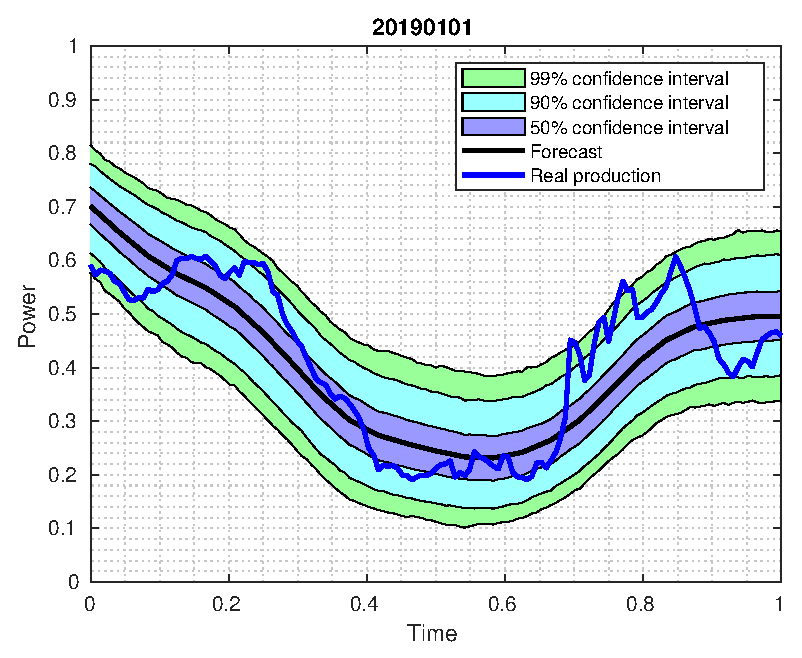
\includegraphics[width=0.3\textwidth]{../../MATLAB_Files/Results/bands_testing_days/optimal_value/1.eps}
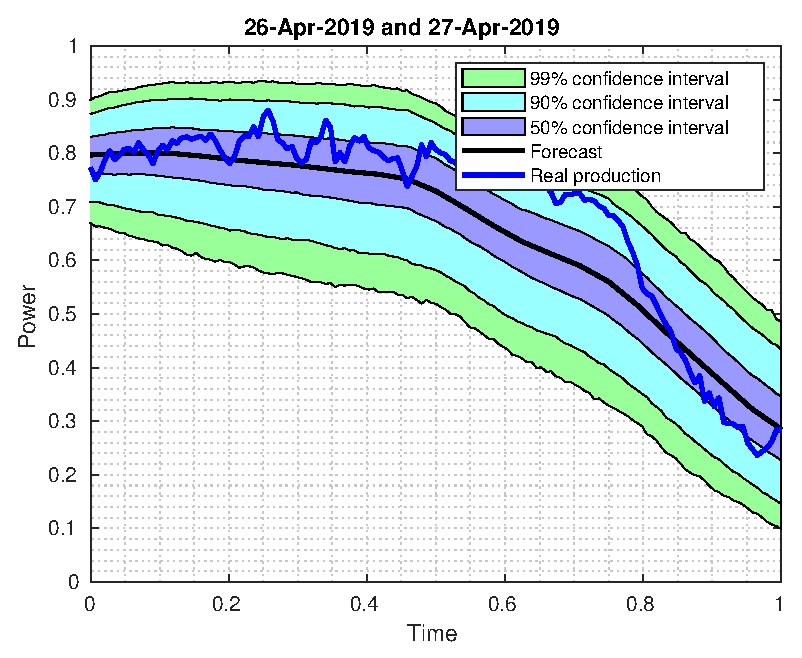
\includegraphics[width=0.3\textwidth]{../../MATLAB_Files/Results/bands_testing_days/optimal_value/2.eps}
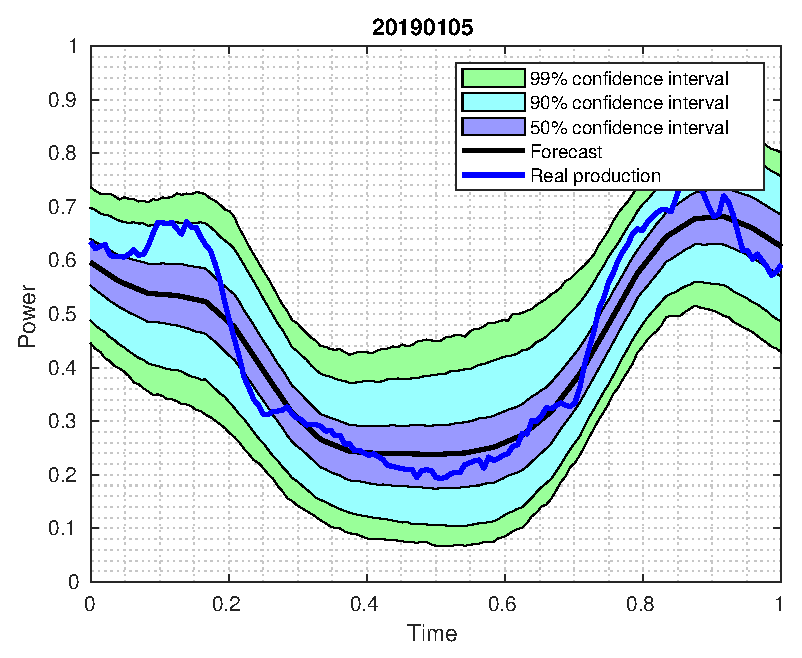
\includegraphics[width=0.3\textwidth]{../../MATLAB_Files/Results/bands_testing_days/optimal_value/3.eps}
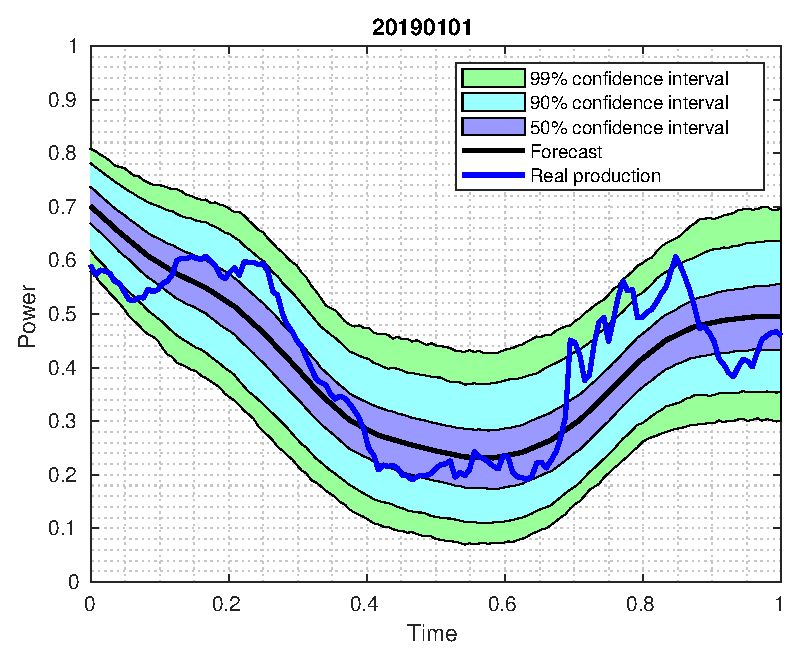
\includegraphics[width=0.3\textwidth]{../../MATLAB_Files/Results/bands_testing_days/Optimal_Lamperti/1.eps}
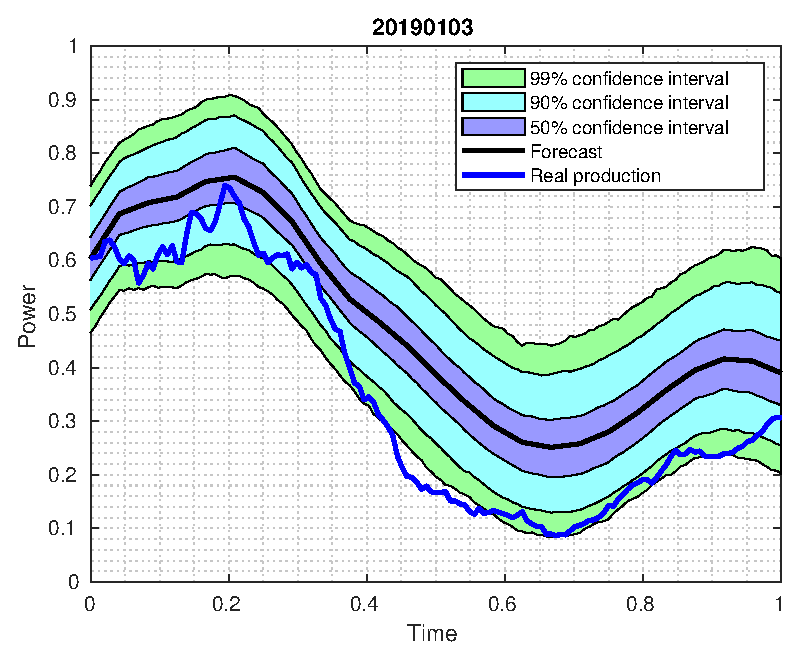
\includegraphics[width=0.3\textwidth]{../../MATLAB_Files/Results/bands_testing_days/Optimal_Lamperti/2.eps}
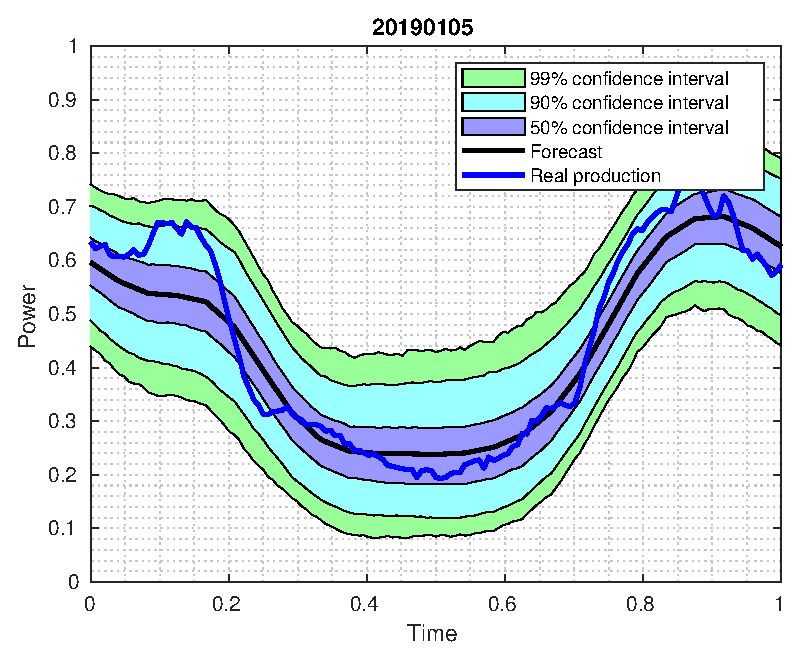
\includegraphics[width=0.3\textwidth]{../../MATLAB_Files/Results/bands_testing_days/Optimal_Lamperti/3.eps}
\end{figure}

\end{frame}

%%%%%%%%%%%%%%%%%%%%%%%%%%%%%%%%%%%%%%%%%%%%%%%%%%%

\setbeamercolor{background canvas}{bg=white!10}
\begin{frame}\frametitle{Simulations over testing days: First row: $(\theta_0^E,\alpha^E)$, second row: $(\theta_0^L,\alpha^L)$}

\begin{figure}[ht!]
\centering
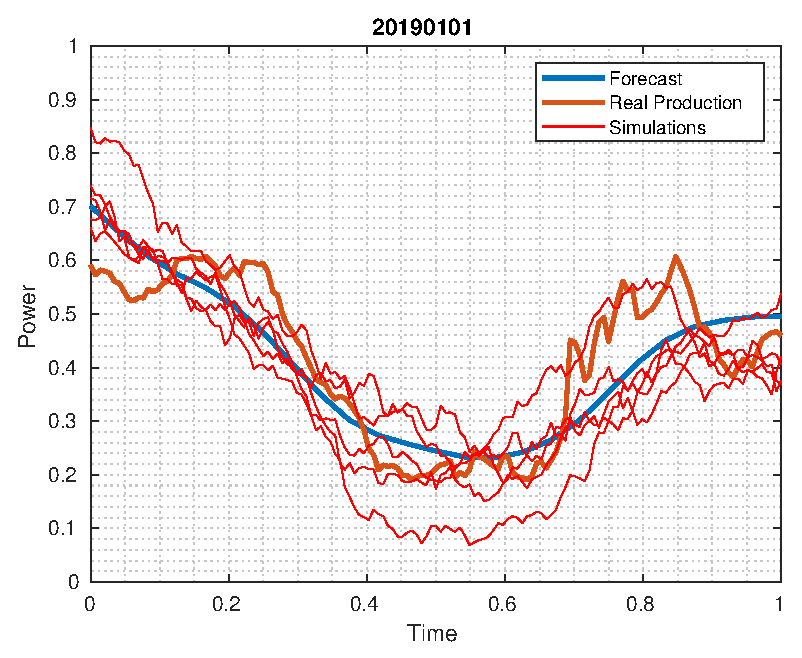
\includegraphics[width=0.3\textwidth]{../../MATLAB_Files/Results/paths_testing_days/optimal_value/1.eps}
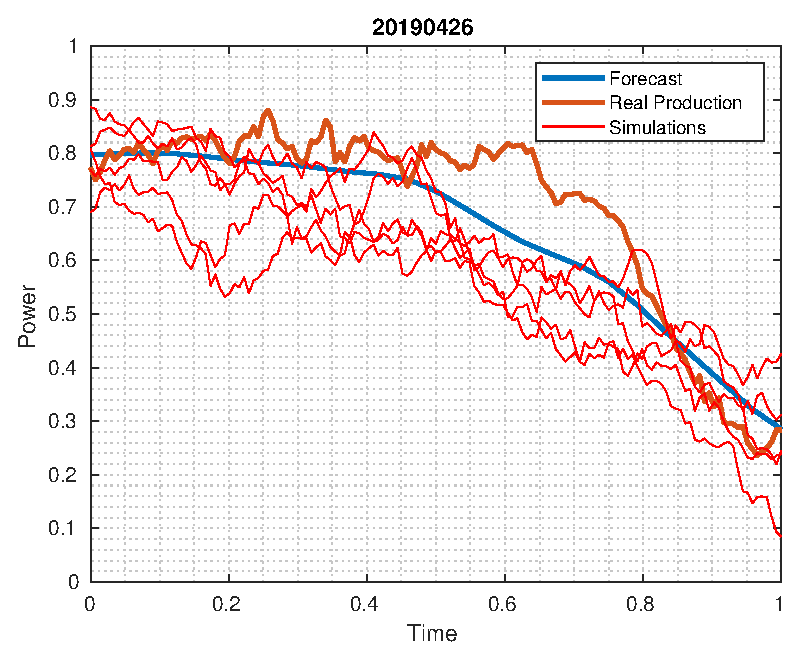
\includegraphics[width=0.3\textwidth]{../../MATLAB_Files/Results/paths_testing_days/optimal_value/2.eps}
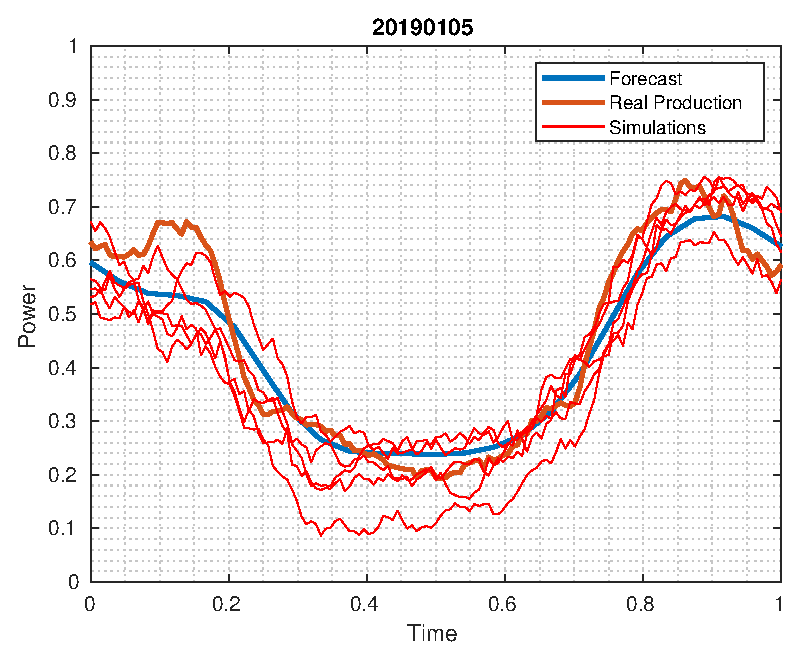
\includegraphics[width=0.3\textwidth]{../../MATLAB_Files/Results/paths_testing_days/optimal_value/3.eps}
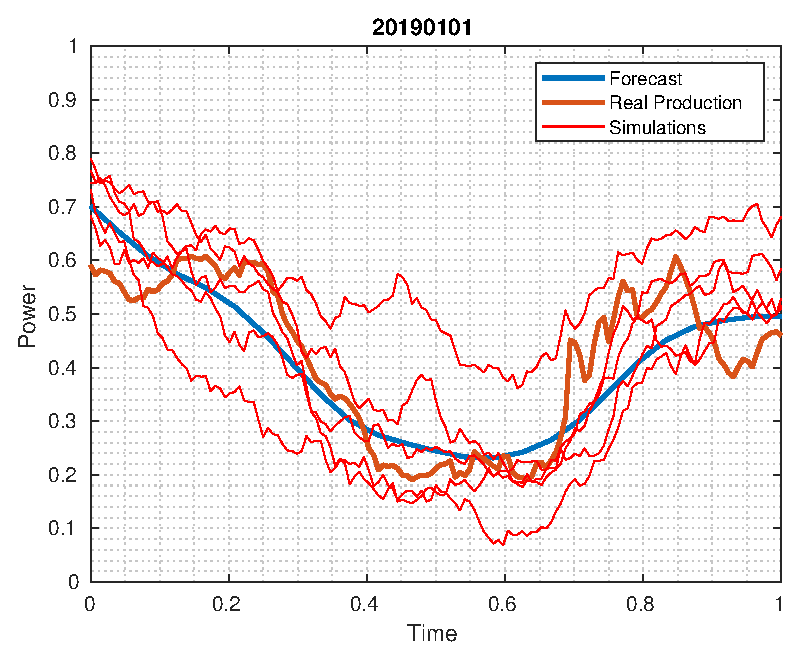
\includegraphics[width=0.3\textwidth]{../../MATLAB_Files/Results/paths_testing_days/Optimal_Lamperti/1.eps}
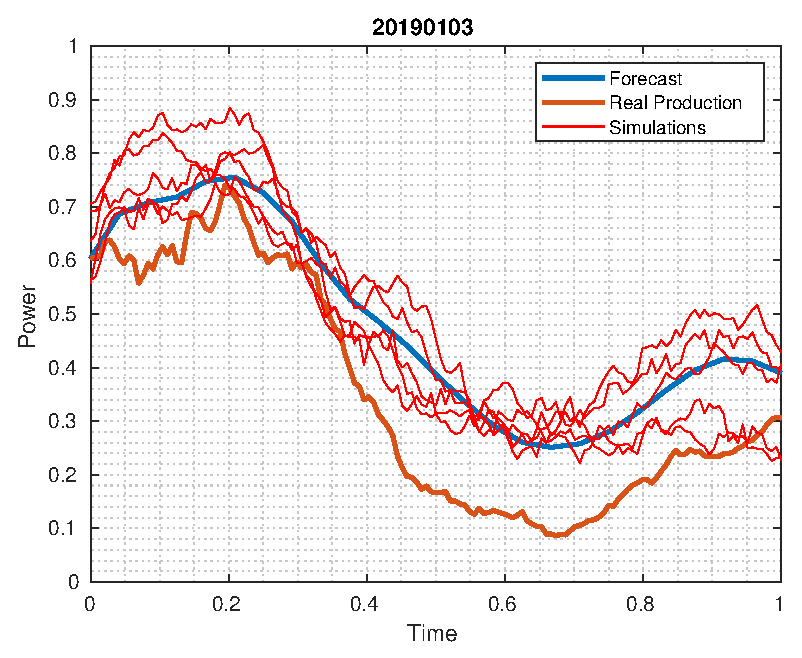
\includegraphics[width=0.3\textwidth]{../../MATLAB_Files/Results/paths_testing_days/Optimal_Lamperti/2.eps}
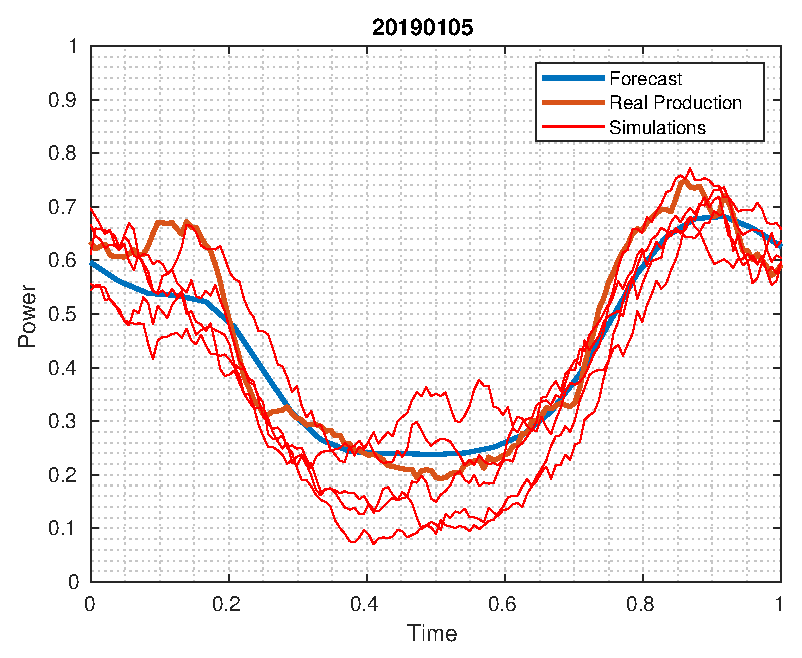
\includegraphics[width=0.3\textwidth]{../../MATLAB_Files/Results/paths_testing_days/Optimal_Lamperti/3.eps}
\end{figure}

\end{frame}

%%%%%%%%%%%%%%%%%%%%%%%%%%%%%%%%%%%%%%%%%%%%%%%%%%%

\setbeamercolor{background canvas}{bg=green!20}
\begin{frame}

{\Huge Other option for Lamperti:}\\
\quad\\
\quad\\
Here we follow \textbf{Likelihood Inference for Discussion: A Survey}, from \textbf{Yacine A\"it-Sahalia}.

\end{frame}

%%%%%%%%%%%%%%%%%%%%%%%%%%%%%%%%%%%%%%%%%%%%%%%%%%%

\setbeamercolor{background canvas}{bg=white!10}
\begin{frame}\frametitle{Density for the error:}

Recall our definitions: $\{\Delta V_i\}_{i=1}^n$ the set of error transitions, $\psi(\theta_0,\alpha,v)$ the Lamperti transform, $\{\Delta Z\}_{i=1}^n$ the transitions after the Lamperti transform, and $\bm{\theta}=(\theta_0,\alpha)$.\\
\quad\\
Our main objective is to estimate the transition density $\rho_V(v|v_0;\bm{\theta})$. Recall from the Lamperti transform definition that $\frac{\dif\psi}{\dif v}(v)=\frac{1}{\sigma(v;\bm{\theta})}$. Then, by the Jacobian formula, we have an expression that related $\rho_V(v|v_0;\bm{\theta})$ and $\rho_Z(z|z_0;\bm{\theta})$:
\begin{equation*}
\rho_V(v|v_0;\bm{\theta})=\frac{\rho_Z(z|z_0;\bm{\theta})}{\sigma(z;\bm{\theta})},
\end{equation*}
where $z=\psi(z;\bm{\theta})$, and we assume that $\rho_Z$ is Gaussian with mean $\mu_Z$ and variance $\sigma_Z^2$ for the random variable $Z$.

\end{frame}

%%%%%%%%%%%%%%%%%%%%%%%%%%%%%%%%%%%%%%%%%%%%%%%%%%%

\setbeamercolor{background canvas}{bg=white!10}
\begin{frame}\frametitle{Density for the error:}

We still have analytic expressions for the moments of the SDE for $V_t$, and we would like to find a relation between this moments, and the mean $\mu_Z$ and variance $\sigma^2_Z$.\\
\quad\\
As $\psi$ and $\sigma$ are not linear, it is not easy to find $E[V]$ and $E[V^2]$ with respect to the density  $\frac{\rho_Z(z|z_0;\bm{\theta})}{\sigma(z;\bm{\theta})}$. If we could find this moments, we would be able to use the MLE directly with the data $\{\Delta V_i\}_{i=1}^n$.\\
\quad\\
One option is to construct empirical moments as a function of $(\theta_0,\alpha,\mu_Z,\sigma_Z)$ with Monte Carlo, and after do the moments matching using this empirical construction.

\end{frame}

\end{document}